\documentclass[botnum]{unmeethesis}
\usepackage{mathtools}
\usepackage{tabularx}
\usepackage{makeidx}  % allows for indexgeneration
\usepackage{amsfonts}
\usepackage{graphicx}
\usepackage{tikz}
\usetikzlibrary{chains,fit,shapes,calc}
\usepackage{verbatim}
\usepackage{semantic}
\usepackage{tabu}
\usepackage{mathptmx}
\usepackage{todonotes}
\usepackage{amsthm}
\usepackage{amssymb}
\usepackage{hyperref}
\usepackage{epigraph}
\usepackage{fontspec}
\usepackage{amsmath}
\usepackage{rotating}
\usepackage{caption}

\setmonofont[Scale=0.8]{DejaVu Sans Mono}

\newcommand{\concat}{\ensuremath{+\!\!\!\!+\,}}  
\newtheorem{thm}{Theorem}
\newtheorem{cor}{Corollary}
\newtheorem{lem}{Lemma}
\newtheorem{theorem}{Theorem}
\newtheorem{lemma}{Lemma}
\newenvironment{proofoutline}
 {\renewcommand\qedsymbol{}\proof[Proof outline]}
 {\endproof}
\def\ce{$\mathcal{\mathcal{C} \mskip -4mu \mathcal{E}} \mskip 4mu$}

\begin{document}

\frontmatter

% Uncomment the next command if you see weird paragraph spacing:
% That is, if you see paragraphs float with lots of white space
% in between them:

% \setlength{\parskip}{0.30cm}

\title{Shared-Environment Call-by-Need}

\author{George Widgery Stelle}

\degreesubject{Ph.D., Computer Science}

\degree{Doctor of Philosophy \\ Computer Science}

\documenttype{Dissertation}

\previousdegrees{B.S., University of British Columbia, 2008 \\
                 M.S., Computer Science, University of New Mexico, 2013}

\date{April, \thisyear}

\maketitle

%\makecopyright

\begin{dedication}
For Beth 
\end{dedication}

\begin{acknowledgments}
  \vspace{1.1in}
  The list of people who deserve acknowledgment for this dissertation is far too
  long to enumerate here. Instead, I'll make a meager attempt at mentioning a
  few who played particularly important roles. 

  Starting at the beginning, I'd like to thank my parents and brothers, who gave
  me a childhood rich in love and fun. In a sense, my decision to pursue a Ph.D.
  was driven by a need to continue having fun doing what I love.  

  Most of the fun I've had has not been sitting and thinking about hard
  problems, but making lifelong friends along the way. To Taylor, Drew, Ben,
  Eric, George, Vu, and others, thank you for the technical discussions, the
  parties, the games, the hikes, the road trips, and most of all your
  friendship. Also, thanks to my three amigos for life, Drake, Mike, and Larkin,
  for the much-needed breaks from work. 

  I thank my Ph.D. advisor, Darko Stefanovic, for his support and advice through
  my unconventional final years through the program. Without his help and
  wisdom there is no question that this dissertation would not exist. Stephanie
  Forrest deserves a great deal of credit as well, both for bringing me into the
  department, and supporting and advising me selflessly through the challenging
  task of finding a topic I love. I would not be here in New Mexico at all
  without the help of my friend Eric Vatikiotis-Bateson. 

  The papers that form this basis of this dissertation would not have been
  possible without the help of my extraordinary co-authors, Darko Stefanovic,
  Stephen Olivier, and Stephanie Forrest. Their ability to write clearly and
  carefully continues to inspire me to be a better communicator. My committee
  members, which include the above co-authors, as well as Kei Davis and Patrick
  Bridges, have my thanks for reviewing my dissertation and sitting through my
  defense. 

  I thank my wonderful wife, Beth, for being my partner in life and always
  inspiring me to be better. And to my children, Adelaide and Sullivan, thank
  you for making life so much more.
\end{acknowledgments}

\maketitleabstract %(required even though there's no abstract title anymore)

\begin{abstract}
Call-by-need semantics formalizes the wisdom that work should be done at most
once. It frees programmers to focus more on the correctness of their code, and
less on the operational details. As a result, programmers of lazy functional
languages rely particularly heavily on their compiler to preserve correctness,
while also relying on the compiler to generate high performance code for high
level abstractions. In this dissertation, I present a novel technique for
compiling call-by-need semantics that uses shared environments to share
results of computation. I show how the approach enables a compiler that
generates high performance code, while staying simple enough to lend itself to
formal reasoning. The dissertation is divided into three main contributions.
First, I present an abstract machine, the \ce machine, which formalizes the
approach.  Second, I show that it can be implemented as a native code compiler
with encouraging performance results.  Finally, I present a verified compiler,
implemented in the Coq proof assistant, demonstrating how the simplicity of
the approach enables formal verification.
\clearpage %(required for 1-pageabstract)
\end{abstract}

\tableofcontents
\listoffigures
%\listoftables

\mainmatter

\chapter{Introduction}\label{chap:intro}
\epigraph{To be admitted to Nature's hearth costs nothing. None is excluded, but
excludes himself. You have only to push aside the curtain.}{\textit{Henry David
Thoreau}}
At the core of this dissertation is a novel technique for implementing call-by-need
semantics. Call-by-need semantics evaluates arguments at call sites \emph{at most
once}. In this way, it combines the advantages of call-by-value which evaluates
arguments exactly once, and call-by-name, which evaluates arguments zero or more
times. The primary insight of this dissertation is that we can implement this
semantics in a natural way using a well known structure in programming language
implementation: the shared environment. 

\section{Motivation}

Like the dissertation as a whole, the motivation is two-fold. First, existing
call-by-need implementations are more eager than necessary about constructing
efficient argument closures. This implies that any under-used argument closure
will have wasted work. Part of the reason this has stayed the case is that it is
not obvious there is a better way. We discuss this motivation in more detail in
Chapter~\ref{chap:cem}. 

The second motivation is that existing call-by-need implementations are complex
in nature, due to their use of supercombinators and flat environments. The STG
machine in particular incorporates many clever techniques for avoiding overheads
of lazy evaluations. While this is useful for generating fast code, it also
makes formal reasoning about the compiler more difficult. This is likely the
primary reason that there aren't existing verified compilers for call-by-need at
the time of this dissertation.

\section{Overview}

This dissertation can be thought of as an exploration of the advantages of
implementing call-by-need with shared environments. There are two advantages to
this approach, corresponding directly to the two motivation points above. First,
it minimizes overheads for thunk creation. It, in a sense, is \emph{lazier}
about lazy evaluation. I take advantage of this by creating a complete native
code compiler for a simple functional language, and showing it has good
performance despite an exceedingly simple implementation. Second, it lends
itself to a exceedingly simple implementation. The simplicity of implementation
allowed investigating some interesting optimizations and implementation
approaches, as well as comparisons with existing implementation approaches, with
only one person doing the development work. Moreover, I show how the simplicity
lets us reason formally to verify the correctness of the implementation.

\section{Call-by-Need}

Because this work is focused on implementing call-by-need semantics, it is worth
spending some time discussing why call-by-need semantics are important. One easy
argument is that call-by-need underlies the widely used programming language
Haskell. Technically, Haskell is a non-strict language. This implies that both
call-by-name and call-by-need are valid implementation strategies. In practice,
there are some situations when one would prefer call-by-name, namely, when
storing an intermediate value is more expensive than re-computing it. These
cases are not limited to call-by-need; call-by-value suffers the same issue.
This implies that in theory, Haskell could switch between call-by-name and
call-by-value depending on the situation. In practice, GHC effectively always
chooses call-by-need, sometimes performing transformations that increase
memoization \cite{jones96floating}.

Even amongst the Haskell community, the advantages and disadvantages of
non-strict evaluation are hotly debated. For example, there exist both
strictness annotations, and even strict-by-default variants of Haskell. There are
real reasons for preferring strict evaluation in some contexts. For example,
memory leaks due to naive attempts at freeing memory are a common issue with
lazy semantics. 

The advantages of non-strict semantics often show up when attempting to write
high level, higher-order abstractions. An example of this principle can be found
in the \texttt{lens} Haskell library. By using laziness everywhere possible, it
ensures that code can compose lenses without introducing nontermination. This is
a strong argument for code re-use advantages in non-strict languages: by using
laziness, one can prevent nontermination everywhere possible without any
additional work. 

In general, the purpose of this dissertation is not to convince the reader that
call-by-need is the ideal semantics. Instead, it takes as a given that it is one
worth spending time on. Finally, I will say that I believe there is a lot of
interesting potential for better understanding the time and space behavior of
non-strict languages. From substructural types to dependent types to control
flow analyses, the field of reasoning about time and space requirements for
higher order languages is still in its infancy, and I am excited to see it
combined with work like that presented here to give developers high confidence
in both their programs' correctness and their time and space requirements. 

\section{Retrospective}

As with any sufficiently large effort, there are places where, if one were to
start over, things would be done differently. An obvious candidate for this
re-writing of history for this dissertation would be \emph{starting} with a
verified compiler, so that the native code compiler itself would be verified.
While noble, this would be a daunting task. Implementing a full native code
compiler is a challenge in itself, but specifying, implementing, and verifying a
compiler, given the current state of verification tools, would be a daunting
undertaking. That said, it would likely have worked to verify and export into
Haskell fragments of the native code compiler. While this would certainly have
been feasible, it would have made modification more difficult. For example,
multiple times through the implementation process, the core language was
extended. Making such core changes in the presence of proofs of correctness
would make for a painful process, something that would have slowed down valuable
time experimenting with the implementation.

\section{Contributions}

There are two primary contributions of my thesis, embodied in the following two
artifacts:

\begin{itemize}
\item A full native code compiler from a simple lazy functional language with
literals and primitive operations to x86\_64 machine code. We show that the
compiler performs comparably to the state of the art on a number of benchmarks.
This implementation and analysis provide evidence supporting the thesis that
shared-environment call-by-need has efficiency benefits over existing
approaches.

\item A verified compiler that compiles from lambda calculus to a simple
instruction machine, along with a specification of correctness and a proof that
the compiler adheres to that specification. The compiler is implemented and the
proofs checked in Coq. This is the first verified compiler of a call-by-need
semantics. This implementation and mechanized proof provides evidence for the
thesis that the simple compiler artifact that arises from shared-environment
call-by-need has benefits for formal reasoning.
\end{itemize}

Combined, these contributions support the core thesis of this dissertation: that
shared-environment call-by-need has valuable contributions to make to the study
and implementation of call-by-need compilers.


\chapter{Background}\label{chap:background}
\epigraph{Science is the belief in the ignorance of experts.}{\textit{Richard
Feynman}}
This chapter provides relevant background for the $\mathcal{\mathcal{C} \mskip
-4mu \mathcal{E}}$ machine and its two implementations, outlining lambda
calculus, evaluation strategies, Curien's calculus of closures, and verifying
implementations in formal logic. 

\section{Preliminaries} \label{sec:prelim}

I begin with the simple lambda calculus ~\cite{barendregt1984lambda}:  $$ t::= x
\; | \;  \lambda x.t \; | \;  t \; t $$ where $x$ is a variable, $\lambda x.t$
is an abstraction, and $t \; t$ is an application. I will primarily use lambda
calculus with deBruijn indices, which replaces variables with a natural number
indexing into the binding lambdas.  This calculus is given by the syntax: $$
t::= i \; | \; \lambda t \; | \; t \; t $$ where $i \in \mathbb{N}$. In both
cases, we use the standard Barendregt syntax conventions, namely that
applications are left associative and the bodies of abstractions extend as far
as possible to the right ~\cite{barendregt1984lambda}.  A \emph{value} in lambda
calculus refers to an abstraction. We are concerned only with evaluation to weak
head normal form (WHNF), which terminates on an abstraction without entering its
body.

In mechanical evaluation of expressions, it would be too inefficient to perform
explicit substitution. To solve this, the standard approach uses closures
~\cite{landin1964mechanical,curien1991abstract,jonesstg,biernacka2007concrete}.
Closures combine a term with an environment, which binds the free variables of
the term to closures. \emph{Entering} a closure refers to the operational
process of beginning to evaluate its term in its environment.

Because of its use of deBruijn indices, I use Curien's calculus of
closures~\cite{curien1991abstract} as the formal basis for closures,
defined in Figure~\ref{fig:curien}. It is a formalization of closures with an
environment represented as a list of closures, indexed by deBruijn indices. We
will occasionally modify this calculus by replacing the deBruijn indices with
variables for readability, in which case variables are looked up in the
environment instead of indexed, e.g., $t[x = c, y = c'])$
~\cite{barendregt1984lambda}. We also add superscript and subscript markers to
denote unique syntax elements, e.g., $t', t_1 \in \textnormal{Term}$. 

\begin{figure}
\textbf{Syntax}
\begin{align*}
\tag{Term} t,v &::= i \; | \; \lambda t \; | \; t \; t  \\
\tag{Variable} i &\in \mathbb{N}  \\
\tag{Closure} c &::= t \left[\rho\right] \\
\tag{Environment} \rho &::= \bullet \; | \; c \cdot \rho \\
\end{align*}
\textbf{Semantics}
\begin{align*}
\inference
{t_1\left[\rho\right] {\Downarrow} \lambda t_2\left[\rho'\right] \\ 
 t_2\left[t_3\left[\rho\right] \cdot \rho'\right] \Downarrow v}
{t_1 t_3\left[\rho\right] \Downarrow v } 
\end{align*}
\begin{align*}
\inference
{c_i \Downarrow v}
{i \left[c_0 \cdot c_1 \cdot ... \cdot c_i \cdot \rho\right] \Downarrow v}
\end{align*}
\begin{align*}
\inference{}{\lambda t\left[\rho\right] \Downarrow \lambda t\left[\rho\right]}
\end{align*}
\caption{Curien's calculus of closures}
\label{fig:curien}
\end{figure}

\section{Evaluation Strategies} \label{sec:eval_strat}

There are three standard evaluation strategies for lambda calculus:
call-by-value, call-by-need, and call-by-name.  Call-by-value evaluates every argument
to a value, whereas call-by-need and call-by-name only evaluate an argument if
it is needed.  If an argument is needed more than once, call-by-name re-computes
the value, whereas call-by-need memoizes the value, so it is computed at most once.
Thus, call-by-need attempts to embody the best of both worlds---never repeat
work (call-by-value), and never perform unnecessary work (call-by-name). These
are intuitively good properties to have, illustrated by the following example,
modified from Danvy et al. ~\cite{danvy2013synthetic}:

$$ \overbrace{c_m (c_m (\cdots(c_m}^{m} \; \mathit{id} \;
\overbrace{\mathit{id})\cdots) \mathit{id})}^{m} \; \mathit{true} \;
\mathit{id} \; \mathit{bottom} $$ where $c_n = \lambda s.\lambda z.\overbrace{s
\; (s \cdots (s}^{n} \; z) \cdots) $, $\mathit{true} = \lambda t.\lambda f.t$,
$\mathit{id}=\lambda x.x$, and \\ $\mathit{bottom} = (\lambda x.x \; x) \lambda x.x \; x$.
When evaluating this expression, call-by-value never terminates, call-by-name
takes exponential time, and call-by-need takes only polynomial time
~\cite{danvy2013synthetic}. Of course, this is a contrived example, but it
illustrates desirable properties of call-by-need.

In practice, however, there are significant performance issues with call-by-need
evaluation.  We focus on the following: \emph{Delaying a computation and
performing it later is slower than performing it immediately.} This deficiency
is well understood \cite{johnsson1984efficient,jonesstg}, and has become part of
the motivation for \emph{strictness analysis}
\cite{mycroft1982abstract,wadler1987projections}, which transforms non-strict
evaluation to strict when possible.

When compiling applications, there are two general implementation approaches.
The first, \emph{eval/apply}, the caller first \emph{evaluates} the function,
then \emph{applies} the arguments to it by knowing its arity. In the second,
\emph{push/enter}, the caller \emph{pushes} the arguments onto the stack, then
\emph{enters} the code that will evaluate to a function \cite{marlow2006making}.  

\section{Existing Call-by-Need Machines}

Diehl et al.~\cite{diehl2000abstract} review the call-by-need
literature in detail.  Here I summarize the most relevant points.

The most well well known and widely used machine for lazy evaluation is the
Spineless Tagless G-Machine (STG machine), which underlies the Glasgow Haskell
Compiler (GHC).  STG uses flat environments that can be allocated on the stack,
the heap, or some combination ~\cite{jonesstg}.  

Two other influential lazy evaluation machines relevant to the \ce 
machine are the call-by-need Krivine machines
~\cite{lkm,krivine2007call,sestoft}, and the three-instruction machine (TIM)
~\cite{TIM}.  Krivine machines started as an approach to call-by-name
evaluation, and were later extended to call-by-need
~\cite{krivine2007call,sestoft,danvy2013synthetic,lkm}.  The \ce machine
modifies the lazy Krivine machine to capture the environment sharing given by
the cactus environment. The TIM is an implementation of call-by-need and
call-by-name ~\cite{TIM}.  It involves, as the name suggests, three machine
instructions, \texttt{TAKE}, \texttt{PUSH}, and \texttt{ENTER}. In
Section~\ref{sec:impl}, I follow Sestoft ~\cite{sestoft} and
re-appropriate these instructions for the \ce machine.

There has also been recent interest in \emph{heapless} abstract
machines for lazy evaluation. Danvy et al. ~\cite{danvy2012inter} and
Garcia et al. ~\cite{garcia2009lazy} independently derived similar
machines from the call-by-need lambda calculus
~\cite{ariola1995call}. These are interesting approaches, but it is not yet
clear how these machines could be implemented efficiently.

\section{Formal Logic} \label{sec:background}

With recent improvements in higher order logics, machine verification of
algorithms has become a valuable tool in software development. Instead of
relying heavily on tests to check the correctness of programs, verification can
prove that algorithms implement their specification for \emph{all} inputs.
Implementing both the specification and the proof in a machine-checked logic
removes the vast majority of bugs found in hand-written proofs, ensuring far
higher confidence in correctness than other standard methods. Other approaches,
such as fuzz testing, have confirmed empirically that verified programs remove
all bugs~\cite{yangfuzz}.

This approach applies particularly well to compilers. Often, the specification
for a compiler is complete: source level semantics for some languages are
exceedingly straightforward to specify, and target architectures have lengthy
specifications that are amenable to mechanization. In addition, writing tests
for compilers that cover all cases is even more hopeless than most domains, due
to the size and complexity of the domain and codomain. The return on investment
is also high: all reasoning about programs compiled with a verified compiler is
provably preserved. 

Likely partially due to the complexities discussed above involved in
implementing lazy languages, among other factors, existing work has focused on
compiling strict languages~\cite{chlipala2007certified, leroy2012compcert,
cakeml14}. Here I use the simple \ce machine as a base for a verified compiler
of a lazy language, using the Coq proof assistant. 

As with many areas of research, the devil is in the details. What exactly does
it mean to claim a compiler is verified?  Essentially, a verified compiler of a
functional language is one that preserves computation of values. That is, we
have an implication: \emph{if the source semantics denotes a value, then the
compiled code computes an equivalent value} \cite{chlipala2007certified}. The
important thing to note is that the implication is only in one direction. If the
source semantics never terminates, this class of correctness theorem says
nothing about the behavior of the compiled code. This has consequences for
Turing-complete source languages. If we are unsure if a source program
terminates, and wish to run it to check experimentally if it does, if we run the
compiled code and it returns a value, we cannot be certain that it corresponds
to a value computed in the source semantics. 

While in theory one could solve this by proving the implication the other
direction, that is, \emph{if the compiled code computes a value then the source
semantics computes an equivalent value}, in practice this is prohibitively
difficult. Effectively, the induction rules for the abstract machine make
constructing such a proof monumentally tricky, as we discuss further in
Chapter~\ref{chap:verified}.

One approach for getting around this issue is to try and capture the divergent
behavior by defining a diverging semantics explicitly \cite{functionalbigstep}.
Then one can safely claim that \emph{if the source semantics diverges according to
our diverging semantics, then the compiled code also diverges}. 

This dissertation takes the approach of Chlipala~\cite{chlipala2007certified}
and defines verification as the first implication above, focusing on the case in
which the source semantics evaluates to a value. This is still a strong
result: any source program that has meaning compiles to an executable with
equivalent meaning. In addition, if anyone ever chooses to augment the language
with a type system that ensures termination, or some notion of progress, then
they could use that in combination with our verification proof for a system that
verifiably supports a wider range of reasoning.

\section{Environment Representations} \label{sec:env}

As mentioned in Section~\ref{sec:prelim}, environments bind free variables to
closures. While any implementation of an environment performs the same function,
there is significant flexibility in how they can be represented. In this section
we review this design space in the context of existing work, both for call by
value and call-by-need.\footnote{Some work refers to this space as
\emph{closure} representation rather than \emph{environment}
representation~\cite{shao1994space,appel1988optimizing}.  Because the term part
of the closure is simply a code pointer and the interesting design choices are
in the environment, I refer to the topic as environment representation. Note
also that global variables are often omitted from environments in real
implementations, we don't consider this implementation detail here.}

There are two common approaches to environment representation: \emph{flat}
environments and \emph{shared} environments (also known as linked
environments)~\cite{appel1988optimizing,shao1994space}. A flat environment is
one in which each closure has its own record of the terms its free variables are
bound to. A shared environment is one in which parts of that record can be
shared among multiple closures~\cite{appel1988optimizing,shao1994space}. For
example, consider the following term: $$(\lambda x.(\lambda y.t_0) (\lambda
z.t_1)) t_2$$ Assuming the term $t_0$ has both $x$ and $y$ as free variables, we
must evaluate it in the environment binding both $x$ and $y$.  Similarly,
assuming $t_1$ contains both $z$ and $x$ as free variables, we must evaluate it
in an environment containing bindings for both $x$ and $z$. Thus, we can
represent the closures for evaluating $t_0$ and $t_1$  as $$t_0[x=t_2[\bullet],
y=c]$$ and $$t_1[x=t_2[\bullet], z=c_1]$$ respectively, where $\bullet$ is the
empty environment.  These are examples of \emph{flat} environments, where each
closure comes with its own record of all of its free variables. Because of the
nested scope of the given term, $x$ is bound to the same closure in the two
environments. Thus, we can also create a shared, linked environment,
represented by the following diagram:

\begin{center}
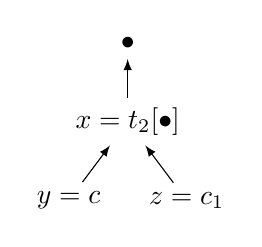
\begin{tikzpicture}[ 
  edge from parent path={(\tikzchildnode\tikzchildanchor) edge [-latex] (\tikzparentnode\tikzparentanchor)},
  level distance=1cm
]
\node (d) {$\bullet$} child{node (a) {$x=t_2[\bullet]$} child{node (b) {$y=c$}} child{node (c)
{$z=c_1$}}};

\end{tikzpicture}
\end{center}
Now each of the environments is represented by a linked list, with the binding
of $x$ shared between them. This is an example of a \emph{shared} environment
~\cite{appel1988optimizing}. This shared, linked structure dates back to the 
first machine for evaluating expressions, Landin's SECD
machine~\cite{landin1964mechanical}.

The drawbacks and advantages of each approach are well known. With a flat
environment, variable lookup can be performed with a simple offset
~\cite{jonesstg,appel1992compiling}. On the other hand, significant
duplication can occur, as I will discuss in Section~\ref{sec:exist}.
With a shared environment, that duplication is removed, but at the cost of
possible link traversal upon dereference. 

As with most topics in compilers and abstract machines, the design space is
actually more complex. For example, Appel and Jim show a wide range of hybrids
~\cite{appel1988optimizing} between the two, and Appel and Shao
~\cite{shao1994space} show an optimized hybrid that aims to achieve the benefits
of both approaches. And as shown in the next section, choice of evaluation
strategy further complicates the picture.

\section{Existing Call-by-Need Environments} \label{sec:exist}

Existing call-by-need machines use flat environments with a heap of
closures~\cite{jonesstg,TIM,johnsson1984efficient,boquist1997grin}. These
environments may contain some combination of primitive values and pointers into the
heap ($p$ below). The pointers and heap implement the memoization of results
required for call-by-need. Returning to the earlier example, $(\lambda
x.(\lambda y.t_0) (\lambda z.t_1)) t_2$, we can view a simplified execution state
for this approach when entering $t_0$ as follows:

\begin{center}
\textbf{Closure}
\begin{align*}
t_0[x=p_0, y=p_1] \\
\end{align*}
\textbf{Heap}
\begin{align*}
p_0 &\mapsto t_2[\bullet] \\
p_1 &\mapsto \lambda z.t_1[x=p_0] 
\end{align*}
\end{center}

Consider $t_2[\bullet]$, the closure at $p_0$. If it is not in WHNF (this sort
of unevaluated closure is called a
\emph{thunk}~\cite{ingerman1961way,peyton1992implementing}), then if it is
entered in either the evaluation of $t_0$ or $t_1$, the resulting value will
overwrite the closure at $p_0$. The result of the computation is then shared
with all other instances of $x$ in $t_0$ and $t_1$. In the case that terms have a
large number of shared variables, environment duplication can be expensive.
Compile-time transformation ~\cite{peyton1992implementing} (tupling arguments)
helps, but we show that the machine can avoid duplication completely.

Depending on $t_0$, either or both of the closures created for its free variables
may not be evaluated. Therefore, it is possible that the work of creating the
environment for that thunk will be wasted. This waste is well known, and
existing approaches address it by avoiding thunks as much as possible
~\cite{jonesstg,johnsson1984efficient}. Unfortunately, in cases like the above
example, thunks are necessary. I aim to minimize the cost of creating such
thunks.

Thunks are special in another way.  Recall that one advantage of flat
environments is quick variable lookups. In a lazy language, this advantage is
reduced because \emph{a thunk can only be entered once}. After it is entered, it
is overwritten with a value, so the next time that heap location is entered it
is entered with a value and a different environment. Thus, the work to ensure
that the variable lookup is fast is used for at most one evaluation of the
thunk. This is in contrast to a call-by-value language, in which every closure
is a value, and can therefore be entered an arbitrary number of times. 

A more subtle drawback of the flat environment representation is that
environments can vary in size, and thus a value in WHNF can be too large to fit
in the space allocated for the thunk it is replacing. This problem is discussed
in Jones et al.~\cite{jonesstg}, where the proposed solution is to put the value
closure in a fresh location in the heap where there is sufficient room. The
original thunk location is then replaced with an indirection to the value at the
freshly allocated location. These indirections are removed during garbage
collection, but do impose some cost, both in runtime efficiency and
implementation complexity.

I have thus far ignored a number of details with regard to current
implementations. For example, the STG machine can split the flat environment, so
that part is allocated on the stack and part on the heap.  The TIM allocates its
flat environments separately from its closures so that each closure is a code
pointer, environment pointer pair~\cite{TIM} while the STG machine keeps
environment and code co-located. Still, the basic design principle holds: a flat
environment for each closure allows quick variable indexing, but with an initial
overhead.

To summarize, the flat environment representation in a call-by-need language
implies that whenever a term might be needed, the necessary environment is
constructed from the current environment.  This operation can be expensive, and
it is wasted if the variable is never dereferenced. In this work, I aim to
minimize this potentially unnecessary overhead.

Figure~\ref{fig:designspace} depicts the design space relevant to this chapter.
There are existing call by value machines with both flat and shared
environments, and call-by-need machines with flat environments. This is the
first work to use a shared environment to implement lazy evaluation. 

It is worth noting that there has been work on lazy machines that effectively use
linked environments, which could potentially be implemented as a shared
environment, e.g., Sestoft's work on Krivine machines~\cite{sestoft}, but none
make the realization that the shared environment can be used to implement
sharing of results, which is the primary contribution of this chapter.

\begin{figure}
\begin{tabularx}{\textwidth}{l | X | X}
                & Flat Environment     & Shared Environment \\ \hline
  Call-by-need  & STG~\cite{jonesstg}, 
                  TIM~\cite{TIM}, 
                  GRIN~\cite{boquist1997grin} 
                & $\mathcal{\mathcal{C} \mskip -4mu \mathcal{E}}$ Machine \\
  Call-by-value & ZAM~\cite{leroy1990zinc}, 
                  SML/NJ~\cite{appel1991standard}
                & ZAM,
                  SECD~\cite{landin1964mechanical}, 
                  SML/NJ \\
\end{tabularx}
\caption{Evaluation strategy and environment structure design space. Each
acronym refers to an existing implementation. Some implementations use multiple
environment representations.}
\label{fig:designspace}
\end{figure}



\chapter{\ce Machine}\label{chap:ce}
\epigraph{The lurking suspicion that something could be simplified is the
world's richest source of rewarding challenges.}{\textit{Edsger Dijkstra}}
In this chapter I define the \ce machine semantics, both big-step and small-step
versions. I try and convey some intuition for why the shared environment
structure works as a technique for sharing results of computation. The
definitions here are the core of both implementations, the native code compiler
in Chapter~\ref{chap:cem} and the verified compiler in
Chapter~\ref{chap:verified}.

Specifically, we formalize the connection between call-by-need evaluation and
shared environments in a big-step semanitcs (Section~\ref{sec:calc}).
Section~\ref{sec:mach} implements the big-step with a small-step semantics by
adding a context (or stack). We leave the proof that it is a correct
implementation for Chapter~\ref{chap:verified}.

\section{Big-Step \ce} \label{sec:calc}

This section shows how the shared environment approach can be applied to
call-by-need evaluation. It starts with a big step semantics that abstracts away
environment representation, Curien's calculus of closures, and then shows how it
can be modified to force sharing. See Curien's call-by-name calculus of closures
in Figure~\ref{fig:curien}. \footnote{Curien calls it a ``lazy'' evaluator, and
there is some ambiguity with the term lazy, but here the term is used only to
mean call-by-need. Curien's condition checking that $i < m$ is omitted as the
semantics is only defined for closed terms.}

The App rule pushes a closure onto the environment, and the Id rule indexes into
the environment, entering the corresponding closure. This section shows that by
removing ambiguity about how the environments are represented, and forcing them
to be represented in a \emph{cactus stack}~\cite{stenstrom1988vlsi}, we can
define a novel call-by-need big step semantics.

To start, consider again the example from Section~\ref{sec:env}, this time with
de Bruijn indices: $(\lambda(\lambda t_0) \; (\lambda t_1)) t_2$.  The terms $t_0$
and $t_1$, when evaluated in Curien's calculus of closures, would have the
following environments, respectively: 

\begin{center}
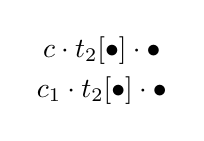
\begin{tikzpicture}
\node {$c \cdot t_2[\bullet] \cdot \bullet$};
\node [yshift=-0.5cm] {$c_1 \cdot t_2[\bullet] \cdot \bullet$};
\end{tikzpicture}
\end{center}

Again, the second closure is identical in each environment.  And again,
we can represent these environments with a shared environment, this time
keeping call-by-need evaluation in mind:
\begin{center}
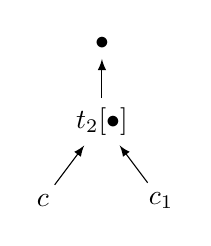
\begin{tikzpicture}[ 
  edge from parent path={(\tikzchildnode\tikzchildanchor) edge [-latex] (\tikzparentnode\tikzparentanchor)},
  level distance=1cm
]
\node (a) {$\bullet$} child{node (d) {$t_2[\bullet]$} child{node (b) {$c$}} child{node (c)
{$c_1$}}};

%\draw let \p1=(a), \p2 =(b), \n1={atan2(\y2-\y1,\x2-\x1)}, \n2={veclen(\y2-\y1,\x2-\x1)}
%  in ($ (a)!0.5!(b) $) ellipse [x radius=\n2/2+10pt, y radius=10pt, rotate=90-\n1];
%\draw let \p1=(a), \p2 =(c), \n1={atan2(\y2-\y1,\x2-\x1)}, \n2={veclen(\y2-\y1,\x2-\x1)}
%  in ($ (a)!0.5!(c) $) ellipse [x radius=\n2/2+10pt, y radius=10pt, rotate=90-\n1];
\end{tikzpicture}
\end{center}
This inverted tree structure seen earlier with the leaves pointing toward the
root is called a \emph{cactus stack} (sometimes called a spaghetti stack or
saguaro stack) when used to implement stacks~\cite{hauck1968burroughs,ichbiah1991rationale}, or a parent pointer tree in
general. In this use case, every node defines an environment as the sequence of
closures in the path to the root.  If $t_2[\bullet]$ is a thunk, and is updated
in place with the value after its first reference, then both environments would
contain the resulting value. This is exactly the kind of sharing that is
required by call-by-need, and thus we can use this structure to build a
call-by-need evaluator. This is the essence of the \ce machine. 

Curien's calculus of closures does not differentiate between flat and shared
environment representations; it has no need to. Therefore, we must derive a new
semantics, forcing the environment to be shared. Because we can hold the closure
directly in the environment, the standard approach of a heap of closures is
replaced with a \emph{heap of environments}. To enforce sharing, we extend
Curien's calculus of closures to explicitly include the heap of environments,
which we refer to as a \emph{cactus environment}. This is effectively a parent
pointer tree in which the contained objects are closures. 

See Figure~\ref{fig:bigstep} for the syntax and semantics of the \ce big step
semantics. Recall that we are only concerned with evaluation of closed terms.
The initial closed term $t$ is placed in a $(t[0],\epsilon[0 \mapsto \bullet])$
configuration, and evaluation terminates on a value. Some shorthand is used to
make heap notation more palatable for both the big-step semantics presented here
and the small step semantics presented in the next section. $\mu(l,i)=l' \mapsto
c \cdot l''$ denotes that looking up the $i$'th element in the linked
environment structure starting at $l$ results in location $l'$, where closure
$c$ and continuing environment $l''$ reside. $\mu(l) = c \cdot l'$ is the
statement that $l \mapsto c \cdot l' \in \mu$, and $\mu(u \mapsto c \cdot l')$
is $\mu$ with location $u$ updated to map to $c \cdot e$. Two 
different semantics are defined, one for call-by-name
(Figure~\ref{fig:bigstepname}) and one for call-by-need
(Figure~\ref{fig:bigstep}), which makes the connection to Curien's call-by-name
calculus more straightfoward. The rule for application is identical for both
semantics: each evaluates the left hand side to a function, then binds the
variable in the cactus environment, extending the current environment.

\begin{figure}
\textbf{Syntax}
\begin{align*}
\tag{Term} t &::= i \; | \; \lambda t \; | \; t \; t  \\
\tag{Variable} i &\in \mathbb{N}  \\
\tag{Closure} c &::= t \left[l\right] \\
\tag{Value} v &::= \lambda t \left[l\right] \\
\tag{Heap} \mu &::= \epsilon \; | \; \mu \left[ l \mapsto \rho \right] \\
\tag{Environment} \rho &::= \bullet \; | \; c \cdot l \\
\tag{Location} l,f &\in \mathbb{N}  \\
\tag{Configuration} s &::= \left(c, \mu \right)
\end{align*}
\textbf{Semantics}
\begin{align*}
\tag{Id} \inference
{\mu \left( l, i \right) = l' \mapsto c \cdot l'' \quad 
 \left(c, \mu\right) \Downarrow \left(v, \mu'\right)}
{\left(i\left[l\right],\mu\right) \Downarrow \left(v, \mu'\right)}
\end{align*} 
\begin{align*}
\tag{App} \inference
{\left(t\left[l\right], \mu\right) \Downarrow \left(\lambda t_2\left[l'\right], \mu'\right) 
   \quad f \not \in \textnormal{dom}\left(\mu'\right)
   \\ \left(t_2\left[f\right], \mu'\left[f \mapsto t_3\left[l\right] \cdot l'\right]\right)
         \Downarrow 
      \left(v, \mu'' \right) 
   }
{\left(t \; t_3\left[l\right], \mu\right) \Downarrow \left(v, \mu'' \right)}  
\end{align*} 
\begin{align*}
\tag{Abs} \inference {} {\left(\lambda t\left[l\right], \mu\right) \Downarrow \left(\lambda t\left[l\right], \mu\right)}
\end{align*}
\caption{Big-step call-by-name \ce syntax and semantics}
\label{fig:bigstepname}
\end{figure}


The only difference between this semantics and Curien's is that if we need
to extend an environment multiple times, the semantics \emph{requires}
sharing it among the extensions. This makes no difference for call-by-name, but
it is needed for the sharing of results in the Id rule. The explicit
environment sharing ensures that the closure that is overwritten with a
value is shared correctly.

\begin{figure}
\textbf{Syntax}
\begin{align*}
\tag{Term} t &::= i \; | \; \lambda t \; | \; t \; t  \\
\tag{Variable} i &\in \mathbb{N}  \\
\tag{Closure} c &::= t \left[l\right] \\
\tag{Value} v &::= \lambda t \left[l\right] \\
\tag{Heap} \mu &::= \epsilon \; | \; \mu \left[ l \mapsto \rho \right] \\
\tag{Environment} \rho &::= \bullet \; | \; c \cdot l \\
\tag{Location} l,f &\in \mathbb{N}  \\
\tag{Configuration} s &::= \left(c, \mu \right)
\end{align*}
\textbf{Semantics}
\begin{align*}
\tag{Id} \inference
{\mu \left( l, i \right) = l' \mapsto c \cdot l'' \quad 
 \left(c, \mu\right) \Downarrow \left(v, \mu'\right)}
{\left(i\left[l\right],\mu\right) \Downarrow \left(v, \mu'\left[l' \mapsto v \cdot l''\right]\right)}
\end{align*}
\begin{align*}
\tag{App} \inference
{\left(t\left[l\right], \mu\right) \Downarrow \left(\lambda t_2\left[l'\right], \mu'\right) 
   \quad f \not \in \textnormal{dom}\left(\mu'\right)
   \\ \left(t_2\left[f\right], \mu'\left[f \mapsto t_3\left[l\right] \cdot l'\right]\right)
         \Downarrow 
      \left(v, \mu'' \right) 
   }
{\left(t \; t_3\left[l\right], \mu\right) \Downarrow \left(v, \mu'' \right)}  
\end{align*}
\begin{align*}
\tag{Abs} \inference {} {\left(\lambda t\left[l\right], \mu\right) \Downarrow \left(\lambda t\left[l\right], \mu\right)}
\end{align*}
\caption{Big-step call-by-need \ce syntax and semantics}
\label{fig:bigstep}
\end{figure}


\section{Small-Step \ce} \label{sec:mach}
Using the big-step \ce from the previous section, we construct a small-step
semantics by adding a stack.  The syntax and semantics are defined in
Figure~\ref{fig:cesm}. 

\begin{figure}
\textbf{Syntax}
\begin{align*}
\tag{State} s &::= \langle c, \sigma, \mu \rangle \\
\tag{Term} t &::= i \; | \; \lambda t \; | \; t \; t  \\
\tag{Variable} i &\in \mathbb{N}  \\
\tag{Closure} c &::= t \left[l\right] \\
\tag{Value} v &::= \lambda t\left[l\right] \\
\tag{Heap} \mu &::= \epsilon \; | \; \mu \left[ l \mapsto \rho \right] \\
\tag{Environment} \rho &::= \bullet \; | \; c \cdot l \\
\tag{Stack} \sigma &::= \square \; | \; \sigma \; c \;  | \; \sigma \; u \\
\tag{Location} l,u,f &\in \mathbb{N}
\end{align*}
\textbf{Semantics}
\begin{align*}
\tag{Upd}
\langle v,  \sigma \; u , \mu \rangle 
  &\rightarrow
\langle v, \sigma, \mu\left(u \mapsto v \cdot l\right) \rangle  
\; \textnormal{where} \; c \cdot l = \mu\left(u\right) \\
\tag{Lam}
\langle \lambda t\left[l\right], \sigma \; c, \mu \rangle 
  &\rightarrow
\langle t\left[f\right], \sigma, \mu\left[f \mapsto c \cdot l\right]\rangle f
\not \in \textnormal{dom}\left(\mu\right)  \\
\tag{App}
\langle t \; t'\left[l\right], \sigma, \mu \rangle
  &\rightarrow
\langle t\left[l\right], \sigma \; t'\left[l\right], \mu \rangle \\
\tag{Var}
\langle i\left[l\right], \sigma, \mu \rangle
  &\rightarrow
\langle c, \sigma \; l'', \mu \rangle
\; \textnormal{where} \; l'' \mapsto c \cdot l' = \mu\left(l, i\right)
\end{align*}
\caption{Small-step \ce syntax and semantics}
\label{fig:cesm}
\end{figure}

The small-step semantics operate identically to the big-step, extended only with
a context (or stack) to implement the updates from the Id subderivation ($\sigma
\; u$) and the operands from the App subderivation ($\sigma \; c$).  Much like
the big-step semantics, a term $t$ is inserted into an initial state $\langle
t[0], \sigma, \epsilon[0\mapsto\bullet]\rangle$ . For the update rule, the
current closure is a value, and there is an update marker as the outermost
context.  This implies that a variable was entered and that the current closure
represents the corresponding value for that variable. Thus, we update the
location $u$ that the variable entered, replacing whatever closure was entered
with the current closure.  The Lam rule takes an argument off the context and
binds it to a variable, allocating a fresh heap location for the bound variable.
This ensures that every instance of the variable will point to this location,
and thus the bound closure will be evaluated at most once. The App rule simply
pushes the argument term in the current environment. The Var rule enters the
closure pointed to by the \textit{i}'th environment location.  

\sloppy To get some intuition for the \ce machine and how it works, please refer
to Figure~\ref{fig:state}, which displays the steps in the evaluation of the
term \\ $(\lambda a.(\lambda b.b \; a) \lambda c.c \; a) \; ((\lambda i.i)
\lambda j.j)$, or $(\lambda(\lambda0\;1)\;\lambda0\;1)\;((\lambda0)\; \lambda0)$
with de Bruijn indices.

\begin{sidewaysfigure}
\begin{align*}
&\langle (\lambda(\lambda0\;1)\;\lambda0\;1)\;((\lambda0)\;\lambda0)[0],\square,\epsilon[0\mapsto\bullet]\rangle\\
&\rightarrow\langle \lambda(\lambda0\;1)\;\lambda0\;1[0],\square (\lambda0)\;\lambda0[0],\epsilon[0\mapsto\bullet]\rangle\\ 
&\rightarrow\langle (\lambda0\;1)\;\lambda0\;1[1],\square,\epsilon[0\mapsto\bullet][1\mapsto(\lambda0)\;\lambda0[0]\cdot0]\rangle\\ 
&\rightarrow\langle \lambda0\;1[1],\square \lambda0\;1[1],\epsilon[0\mapsto\bullet][1\mapsto(\lambda0)\;\lambda0[0]\cdot0]\rangle\\ 
&\rightarrow\langle 0\;1[2],\square,\epsilon[0\mapsto\bullet][1\mapsto(\lambda0)\;\lambda0[0]\cdot0][2\mapsto\lambda0\;1[1]\cdot1]\rangle\\ 
&\rightarrow\langle 0[2],\square 1[2],\epsilon[0\mapsto\bullet][1\mapsto(\lambda0)\;\lambda0[0]\cdot0][2\mapsto\lambda0\;1[1]\cdot1]\rangle\\ 
&\rightarrow\langle \lambda0\;1[1],\square 1[2] 2,\epsilon[0\mapsto\bullet][1\mapsto(\lambda0)\;\lambda0[0]\cdot0][2\mapsto\lambda0\;1[1]\cdot1]\rangle\\ 
&\rightarrow\langle \lambda0\;1[1],\square 1[2],\epsilon[0\mapsto\bullet][1\mapsto(\lambda0)\;\lambda0[0]\cdot0][2\mapsto\lambda0\;1[1]\cdot1]\rangle\\ 
&\rightarrow\langle 0\;1[3],\square,\epsilon[0\mapsto\bullet][1\mapsto(\lambda0)\;\lambda0[0]\cdot0][2\mapsto\lambda0\;1[1]\cdot1][3\mapsto1[2]\cdot1]\rangle\\ 
&\rightarrow\langle 0[3],\square 1[3],\epsilon[0\mapsto\bullet][1\mapsto(\lambda0)\;\lambda0[0]\cdot0][2\mapsto\lambda0\;1[1]\cdot1][3\mapsto1[2]\cdot1]\rangle\\ 
&\rightarrow\langle 1[2],\square 1[3] 3,\epsilon[0\mapsto\bullet][1\mapsto(\lambda0)\;\lambda0[0]\cdot0][2\mapsto\lambda0\;1[1]\cdot1][3\mapsto1[2]\cdot1]\rangle\\ 
&\rightarrow\langle 0[1],\square 1[3] 3,\epsilon[0\mapsto\bullet][1\mapsto(\lambda0)\;\lambda0[0]\cdot0][2\mapsto\lambda0\;1[1]\cdot1][3\mapsto1[2]\cdot1]\rangle\\ 
\end{align*}
\caption{Small-step \ce example. Evaluation of
$(\lambda(\lambda0\;1)\;\lambda0\;1)\;((\lambda0)\;\lambda0)$}
\end{sidewaysfigure}

\begin{sidewaysfigure}
\ContinuedFloat
\begin{align*}
&\rightarrow \langle (\lambda0)\;\lambda0[0],\square 1[3] 3 1,\epsilon[0\mapsto\bullet][1\mapsto(\lambda0)\;\lambda0[0]\cdot0][2\mapsto\lambda0\;1[1]\cdot1][3\mapsto1[2]\cdot1]\rangle\\ 
&\rightarrow \langle \lambda0[0],\square 1[3] 3 1 \lambda0[0],\epsilon[0\mapsto\bullet][1\mapsto(\lambda0)\;\lambda0[0]\cdot0][2\mapsto\lambda0\;1[1]\cdot1][3\mapsto1[2]\cdot1]\rangle\\ 
&\rightarrow\langle 0[4],\square 1[3] 3 1,\epsilon[0\mapsto\bullet][1\mapsto(\lambda0)\;\lambda0[0]\cdot0][2\mapsto\lambda0\;1[1]\cdot1][3\mapsto1[2]\cdot1][4\mapsto\lambda0[0]\cdot0]\rangle\\ 
&\rightarrow\langle \lambda0[0],\square 1[3] 3 1 4,\epsilon[0\mapsto\bullet][1\mapsto(\lambda0)\;\lambda0[0]\cdot0][2\mapsto\lambda0\;1[1]\cdot1][3\mapsto1[2]\cdot1][4\mapsto\lambda0[0]\cdot0]\rangle\\ 
&\rightarrow\langle \lambda0[0],\square 1[3] 3 1,\epsilon[0\mapsto\bullet][1\mapsto(\lambda0)\;\lambda0[0]\cdot0][2\mapsto\lambda0\;1[1]\cdot1][3\mapsto1[2]\cdot1][4\mapsto\lambda0[0]\cdot0]\rangle\\ 
&\rightarrow\langle \lambda0[0],\square 1[3] 3,\epsilon[0\mapsto\bullet][1\mapsto\lambda0[0]\cdot0][2\mapsto\lambda0\;1[1]\cdot1][3\mapsto1[2]\cdot1][4\mapsto\lambda0[0]\cdot0]\rangle\\ 
&\rightarrow\langle \lambda0[0],\square 1[3],\epsilon[0\mapsto\bullet][1\mapsto\lambda0[0]\cdot0][2\mapsto\lambda0\;1[1]\cdot1][3\mapsto\lambda0[0]\cdot1][4\mapsto\lambda0[0]\cdot0]\rangle\\ 
&\rightarrow\langle 0[5],\square,\epsilon[0\mapsto\bullet][1\mapsto\lambda0[0]\cdot0][2\mapsto\lambda0\;1[1]\cdot1][3\mapsto\lambda0[0]\cdot1][4\mapsto\lambda0[0]\cdot0][5\mapsto1[3]\cdot0]\rangle\\ 
&\rightarrow\langle 1[3],\square 5,\epsilon[0\mapsto\bullet][1\mapsto\lambda0[0]\cdot0][2\mapsto\lambda0\;1[1]\cdot1][3\mapsto\lambda0[0]\cdot1][4\mapsto\lambda0[0]\cdot0][5\mapsto1[3]\cdot0]\rangle\\ 
&\rightarrow\langle 0[1],\square 5,\epsilon[0\mapsto\bullet][1\mapsto\lambda0[0]\cdot0][2\mapsto\lambda0\;1[1]\cdot1][3\mapsto\lambda0[0]\cdot1][4\mapsto\lambda0[0]\cdot0][5\mapsto1[3]\cdot0]\rangle\\ 
&\rightarrow\langle \lambda0[0],\square 5 1,\epsilon[0\mapsto\bullet][1\mapsto\lambda0[0]\cdot0][2\mapsto\lambda0\;1[1]\cdot1][3\mapsto\lambda0[0]\cdot1][4\mapsto\lambda0[0]\cdot0][5\mapsto1[3]\cdot0]\rangle\\ 
&\rightarrow\langle \lambda0[0],\square 5,\epsilon[0\mapsto\bullet][1\mapsto\lambda0[0]\cdot0][2\mapsto\lambda0\;1[1]\cdot1][3\mapsto\lambda0[0]\cdot1][4\mapsto\lambda0[0]\cdot0][5\mapsto1[3]\cdot0]\rangle\\ 
&\rightarrow\langle \lambda0[0],\square,\epsilon[0\mapsto\bullet][1\mapsto\lambda0[0]\cdot0][2\mapsto\lambda0\;1[1]\cdot1][3\mapsto\lambda0[0]\cdot1][4\mapsto\lambda0[0]\cdot0][5\mapsto\lambda0[0]\cdot0]\rangle
\end{align*}
\caption{Small-step \ce example. Evaluation of
$(\lambda(\lambda0\;1)\;\lambda0\;1)\;((\lambda0)\;\lambda0)$ (cont.)}
\label{fig:state}
\end{sidewaysfigure}



\chapter{Native Code Compilation}\label{chap:cem}
\epigraph{Much of my work has come from being lazy.}{\textit{John Backus}}
Existing implementations of call-by-need take care in \emph{packaging} a delayed
computation, or \emph{thunk}, by building a closure with an array that contains
the bindings of all free variables \cite{jonesstg,boquist1997grin}. The overhead
induced by this operation is well known, and is one reason existing
implementations avoid thunks wherever possible \cite{johnsson1984efficient}. The
key insight of our Cactus Environment (\ce) Machine is that this overhead can be
minimized by only recording a location in a shared environment.

As an example, consider the application $f \; e$. In existing call-by-need
implementations, e.g., the STG machine\cite{jonesstg}, a closure with a flat
environment will be constructed for $e$.  Doing so incurs a time and memory cost
proportional to the number of free variables of $e$. \footnote{In some
implementations, these are lambda-lifted to be formal parameters, but the
principle is the same.} We minimize this packaging cost by recording a
location in a shared environment, which requires only two
machine words (and two instructions) for the thunk: one for the code pointer,
and one for the environment pointer. One way to think about the approach is that
it is \emph{lazier} about lazy evaluation: in the case that $e$ is unneeded, the
work to package it in a thunk is entirely wasted. In the spirit of lazy
evaluation, we attempt to minimize this potentially unnecessary work.  

In this chapter we present a simple implementation of the \ce machine that
compiles a simple lazy functional language to x86\_64 assembly. In addition, it
presents a preliminary evaluation that shows performance comparable to existing
implementations (Sections~\ref{sec:impl} and~\ref{sec:eval}). 

We describe a straightforward
implementation of \ce in Section~\ref{sec:impl}, extended with machine literals
and primitive operations, and compiling directly to native code. We evaluate the
implementation in Section~\ref{sec:eval}, showing that it is capable of
performing comparably to existing implementations despite lacking several common
optimizations, and we discuss the results. We discuss related work, the
limitations of our approach, and some ideas for future work in
Section~\ref{sec:disc}.

\input{tfp16/implement}
\input{tfp16/evaluation}
\input{tfp16/results}
\section{Discussion and Related Work} \label{sec:disc}

This section compares the compiler presented in this chapter with existing work,
and discusses areas for future work.

\subsection{Closure Representation}
Appel and Shao \cite{shao1994space} and Appel and Jim \cite{appel1988optimizing}
both cover the design space for closure representation, and develop an approach
called \emph{safely linked closures}. The approach uses flat closures when
there is no duplication, and links in a way that preserves liveness, to prevent
violation of the \emph{safe for space complexity} (SSC) rule
\cite{shao1994space}. While I do not address SSC or garbage collection in
general, understanding the relationship between SSC and shared environment
call-by-need is an interesting area for future work. In particular, hot
environments with no sharing could benefit greatly from replacing shared
structure with flat.

\subsection{Eval/Apply vs. Push/Enter}
Marlow and Peyton Jones describe two approaches to the implementation of
function application: eval/apply, where the function is evaluated and then
passed the necessary arguments, and push/enter, where the arguments are pushed
onto the stack and the function code is entered \cite{marlow2006making}. They
conclude that despite push/enter being a standard approach to lazy machines,
eval/apply performs better. While our current approach uses push/enter,
investigating whether eval/apply could be usefully implemented for a shared
environment machine like the $\mathcal{\mathcal{C} \mskip -4mu \mathcal{E}}$
machine is an interesting avenue for future work.

\subsection{Collapsed Markers}
Friedman et al.\ show how a machine can be designed to prevent multiple adjacent
update markers being pushed onto the stack \cite{lkm}.  This property is
desirable because multiple adjacent update markers are always updated with the
same value. They give examples showing that in some cases, these redundant
update markers can cause an otherwise constant-space stack to overflow.  They
implement an optimization that collapses update markers by adding a layer of
indirection between heap locations and closures. A similar approach,
but without the performance hit caused by an extra layer of indirection should
be possible, as follows: upon a variable dereference the $\mathcal{\mathcal{C}
\mskip -4mu \mathcal{E}}$ machine checks if the top of the stack is an update.
If it is, instead of pushing a redundant update marker onto the stack, the
machine replaces the closure in the heap at the marker location with an update
marker pointing to the location specified by the marker on the top of the stack.
Then, the variable dereference rule checks if there is an update marker instead
of a closure in the dereferenced cell, and if there is, then the value closure
pointed to by that update marker will be copied, overwriting the update marker.
This effectively makes the update mechanism lazier, only updating one marker
eagerly, and any equivalent markers on demand.  We leave this optimization for
future work.

\subsection{Register Allocation} \label{sec:alloc}
One advantage of flat environments is that register allocation is
straightforward \cite{appel1992compiling,jonesstg,terei2010llvm}. It is less
obvious how to do register allocation with the $\mathcal{\mathcal{C} \mskip
-4mu \mathcal{E}}$ machine.  

One possible approach that could work well with our shared environment approach
would be to only load free variables into registers that are statically known to
be needed. In other words, some environment variables may not be used, so only
those that will definitely be used should be loaded into registers when a
closure is entered, while the rest could be loaded on demand from memory.

\subsection{Characterizing Performance}
While we have provided a few benchmarks and some intuition for why the shared
environments would be preferable in some situations, we haven't really
characterized when programs will benefit from the approach.  This, along with
the joining of shared and flat environments, is left for future work. It will
likely require a combination of careful performance profiling, static analysis
tools, and a deeper understanding of the performance tradeoffs discussed in the
Chapter.



\chapter{Verified Compilation}\label{chap:verified}
\epigraph{I don't believe in empirical science. I only believe in a priori
truth.}{\textit{Kurt Gödel}}

\label{sec:introduction}
As discussed in Chapter~\ref{chap:intro}, lazy functional programming languages
like Haskell lend themselves particularly well to reasoning about correctness.
It is for this reason we should be motivated to build a verified compiler for a
call-by-need semantics, the default semantics for lazy functional languages: we
want this reasoning to be preserved.  Unfortunately, one of the challenges for
formalization of non-strict compilers is that the semantics of call-by-need
abstract machines tend to be complex, incorporating complex optimizations into
the semantics, requiring preprocessing of terms, and closures of variable sizes
\cite{jonesstg, TIM}.  In this chapter, we use the \ce machine \cite{cem},
taking advantage of its simplicity to ease the formal reasoning burden that goes
with building a verified compiler.

Verified compilers provide powerful guarantees about the code they generate and
its relation to the corresponding source code \cite{chlipala2007certified,
leroy2012compcert, cakeml14}.  In particular, for higher order functional
languages, they ensure that the non-trivial task of compiling lambda
calculus and its extensions to machine code is implemented correctly,
preserving source semantics. The amortized return on investment for verified
compilers is high: any reasoning about any program which is compiled with a
verified compiler is provably preserved. 

Existing verified compilers have focused on call-by-value semantics
\cite{chlipala2007certified, leroy2012compcert, cakeml14}. This semantics has
the property of being historically easier to implement than call-by-need, and
therefore likely easier to reason about formally. In this chapter, formalize the
\ce machine described in Chapter 2. We use the Coq proof assistant
\cite{barras1997coq} to implement and prove the correctness of our compiler. We
start with a source language of $\lambda$ calculus with de Bruijn indices:
\begin{align*}
 t &::= t \; t \; | \; x \; | \;  \lambda \; t \\
 x &\in \mathbb{N}
\end{align*}
Our source semantics is the big-step operational semantics of the \ce 
machine, which uses shared environments to share results between instances of a
bound variable. To strengthen the result, and relate it to a better-known
semantics, we also show that the call-by-name \ce machine implements
Curien's call-by-name calculus of closures. 

It may surprise the reader to see that we do not start with a better known
call-by-need semantics; we address this concern in
Section~\ref{sec:discussion}.  We hope that the proof of compiler correctness,
along with the proof that our call-by-name version of the semantics implements
Curien's call-by-name semantics, convinces the reader that we have indeed
implemented a call-by-need semantics, despite not using a better known
definition of call-by-need. 

For our target, we define a simple instruction machine, described in
Section~\ref{sec:im_semantics}. This simple target allows us to describe the
compiler and proofs concisely for the chapter, while still allowing
flexibility in eventually verifying a compiler down to machine code for some
set of real hardware, e.g., x86, ARM, or Power. 

Our main results is a proof that whenever the source semantics evaluates to a
value, the compiled code evaluates to the same value. While there are stronger
definitions of what qualifies as a verified compiler, we argue that this is
sufficient in Section~\ref{sec:discussion}. This main result, along with the
proof that the call-by-name version of our semantics implements Curien's
calculus of closures, are the primary contributions of this chapter. We are
unaware of any existing verified non-strict compilers, much less a verified
compiler of call-by-need. 

The chapter is structured as follows. In Section~\ref{sec:background} we give the
necessary background. In Section~\ref{sec:cem_big} we describe the source syntax
and semantics (the big-step \ce semantics) in detail.  We also use
this section to define a call-by-name version of the semantics, and
show that it implements Curien's calculus of closures \cite{curien1991abstract}.  In
Section~\ref{sec:cem_small} we describe the small-step \ce semantics
and its relation to the big-step semantics. In Section~\ref{sec:im_semantics}
we describe the instruction machine syntax and semantics. In
Section~\ref{sec:compiler} we describe the compilation from machine terms to
assembly language. In Section~\ref{sec:correctness} we describe how the evaluation
of compiled programs is related to the small-step \ce semantics. We
compose this proof with the proof that the small-step semantics implement the
big-step semantics to show that the instruction machine implements the big-step
semantics. In Section~\ref{sec:discussion} we discuss threats to validity,
future work, and related work. The Coq source code with all the definitions and
proofs described in this document is available at
\url{https://github.com/stelleg/cem\_coq}. 

\input{ifl18/cem}
\section{Small-Step \ce} \label{sec:cem_small}

In this section I review the small-step semantics of the \ce 
machine, and show that it implements the big-step semantics of
Section~\ref{sec:cem_big}. This is a fairly straightforward transformation implemented
by adding a stack. The source language is the same, and I simply add a stack to
our configuration (and call it a state). The stack elements are either argument
closures or update markers. Update markers are pushed onto the stack when a
variable dereferences that location in the heap. When they are popped by an
abstraction, the closure at that location is replaced by said abstraction, so
that later dereferences by the same variable in the same scope dereference the
value, and do not repeat the computation.  Argument closures are pushed onto the
stack by applications, with the same environment pointer duplicated in the
current closure and the argument closure.  Argument closures are popped off the
stack by abstractions, which allocate a fresh memory location, write the
argument closure to it, write the environment continuation as the current
environment pointer, then enter the body of the abstraction with the fresh
environment pointer. This is the mechanism used for extending the shared
environment structure. The semantics is defined formally in
Figure~\ref{fig:cesm}.  

\subsection{Relation to Big Step} \label{sec:cem_cesm}
Here I prove that the small-step semantics implements the big-step semantics of
Section~\ref{sec:cem_big}. This requires first a notion of reflexive transitive closure,
which I define in the standard way. We also make use of the fact that the
reflexive transitive closure can be defined equivalently to extend from the left
or right. 

\begin{lemma}
If the big-step semantics evaluates from one configuration to another, then the
reflexive transitive closure of the small-step semantics evaluates from the same
starting configuration with any stack to the same value configuration with that
same stack.
\end{lemma}
\begin{proofoutline}
The proof proceeds by induction on the big-step relation. We define our
induction hypothesis so that it holds for all stacks, which gives us the
desired case of the empty stack as a simple specialization. The rule for
abstractions is the trivial base case. Var rule applies as the first step, and
the induction hypothesis applies to the stack with the update marker on it. To
ensure that the Upd rule applies I use the fact that the big-step semantics
only evaluates to abstraction configurations, and the fact that the reflexive
transitive closure can be rewritten with steps on the right. For the Application
rule, I take advantage of the fact that one can append two evaluations together,
as well as extend a reflexive transitive closure from the left or the right. As
with the Var rule I use the fact that the induction rule is defined for all
stacks to ensure evaluation of the left hand side to a value with the argument
on the top of the stack. Finally, I extend the environment with the argument
closure, and evaluate the result to a value by the second induction hypothesis.
\end{proofoutline}

Adding a stack in this fashion is a standard approach to converting between big
step and small-step semantics, and applies here in a straightforward way. 

\input{ifl18/im}
\section{Compiler} \label{sec:compiler}

In this section we describe the compiler, which compiles lambda terms with
de Bruijn indices to programs. The compiler proceeds by recursion on lambda
terms, keeping a current index into the program to ensure correct linking
without a separate pass. For variables, when we get to zero we push the current
environment pointer and a null instruction pointer to denote the update marker
to the location of the closure being entered. Then we $\mathit{mov}$ the closure
at that location into $r1$ and $ep$, and $\mathit{jump}$ to
$r1$, recalling that the $\mathit{jump}$ sets the $ip$. For 
nonzero variables, we replicate traversing the environment pointer $i$
times before loading the closure.  For applications, we calculate the program
location of the argument basic block, and push that and the current environment
pointer onto the stack, effectively pushing an argument closure on top of the
stack. We then $\mathit{jump}$ to the left hand side of the application, as is
standard for push-enter evaluation. For abstractions, we use a conditional jump
depending on whether the top of the stack is a null pointer (and therefore an
update marker) or a valid instruction pointer (and therefore an argument). If it
is an update marker, we update the heap location defined by the update marker
with the current value instruction pointer and the current environment pointer.
We must point to the first of the three abstractions basic blocks, as this value
could later update another heap location as well. In the case that the top of
the stack was a valid instruction pointer, we allocate a new chunk of 3 word of
memory, and $\mathit{mov}$ the argument closure into it, with the current
environment pointer as the environment continuation. We then set our current
environment pointer to this fresh location. This is the process by which we
extend our shared environment structure in the instruction machine. Finally, we
perform an unconditional jump to the next basic block, which is the first basic
block of the compiled body of the lambda. As this is an unconditional jump to
the next basic block, for real machine code this jump can be omitted. 

\begin{figure}
\begin{align*}
\mathit{var} \; 0 :=  \;
  &\mathit{push} \; ep : \\
  &\mathit{push} \; 0 : \\
  &\mathit{mov} \; \left(ep\%0\right) \; r1 : \\
  &\mathit{mov} \; \left(ep\%1\right) \; ep : \\
  &\mathit{jump} \; r1 \\
\mathit{var} \; \left(i+1\right) := \;
  &\mathit{mov} \; \left(ep\%2\right) \; ep : \\
  &\mathit{var} \; i \\
\mathit{compile} \; i \; k := \; & \left[\mathit{var} \; i\right] \\
\mathit{compile} \; \left( m \; n \right) \; k := \;
  &\mathit{let} \; ms = \mathit{compile} \; m \; \left(k+1\right) \; in \\
  &\mathit{let} \; nk = 1+k+length \; ms \; in \\
  &\mathit{push} \; ep :  \\
  &\mathit{push} \; nk : \\
  &\mathit{jump} \; \left(k+1\right) :: \\
  &ms \concat \mathit{compile} \; n \; nk \\
\mathit{compile} \; \left(\lambda b\right) \; k := \;
  &\mathit{pop} \; r1 : \\
  &\mathit{jump} \; \left(r1, k+1 \right) \; \left(k+2\right) :: \\
  &\mathit{pop} \; r1 : \\
  &\mathit{mov} \; k \; r1\%0 : \\
  &\mathit{mov} \; ep \; r1\%1 : \\
  &\mathit{jump} \; k :: \\
  &\mathit{new} \; 3 \; r2 : \\
  &\mathit{mov} \; r1 \; \left(r2\%0\right) : \\
  &\mathit{pop} \; \left(r2\%1\right) : \\
  &\mathit{mov} \; ep \; \left(r2\%2\right) : \\
  &\mathit{mov} \; r2 \; ep : \\
  &\mathit{jump} \; \left(k+3\right) :: \\
  &\mathit{compile} \; b \; \left(k+3\right)
\end{align*}
\caption{Compiler Definition}
\label{fig:compiler}
\end{figure}

Being able to define the full compiler this simply is crucial to this
verification project. Other, more sophisticated implementations of call-by-need,
such as the STG machine, are much harder to implement and reason about. It is
worth noting that despite this simplicity, initial tests suggest that performance
is reasonable, and is often competitive with state of the art
(Chapter~\ref{chap:cem}). 

As with the relation discussed in Section~\ref{sec:cem_big}, a term does not
have to be closed to compile it. Indeed, we will happily generate code that if
entered, will attempt to dereference the null pointer, leaving the machine
stuck. Because we are only concerned with proving that the source semantics are
implemented in the case that it evaluates to a value, this is not a problem. If
we wanted a more general theorem, we could try to show that if the source
semantics gets stuck trying to dereference a free variable, the implementation
would get stuck in the same way, both failing to dereference a null pointer.  

\input{ifl18/correctness}
\section{Discussion and Related Work} \label{sec:disc}

This section compares the compiler presented in this chapter with existing work,
and discusses areas for future work.

\subsection{Closure Representation}
Appel and Shao \cite{shao1994space} and Appel and Jim \cite{appel1988optimizing}
both cover the design space for closure representation, and develop an approach
called \emph{safely linked closures}. The approach uses flat closures when
there is no duplication, and links in a way that preserves liveness, to prevent
violation of the \emph{safe for space complexity} (SSC) rule
\cite{shao1994space}. While I do not address SSC or garbage collection in
general, understanding the relationship between SSC and shared environment
call-by-need is an interesting area for future work. In particular, hot
environments with no sharing could benefit greatly from replacing shared
structure with flat.

\subsection{Eval/Apply vs. Push/Enter}
Marlow and Peyton Jones describe two approaches to the implementation of
function application: eval/apply, where the function is evaluated and then
passed the necessary arguments, and push/enter, where the arguments are pushed
onto the stack and the function code is entered \cite{marlow2006making}. They
conclude that despite push/enter being a standard approach to lazy machines,
eval/apply performs better. While our current approach uses push/enter,
investigating whether eval/apply could be usefully implemented for a shared
environment machine like the $\mathcal{\mathcal{C} \mskip -4mu \mathcal{E}}$
machine is an interesting avenue for future work.

\subsection{Collapsed Markers}
Friedman et al.\ show how a machine can be designed to prevent multiple adjacent
update markers being pushed onto the stack \cite{lkm}.  This property is
desirable because multiple adjacent update markers are always updated with the
same value. They give examples showing that in some cases, these redundant
update markers can cause an otherwise constant-space stack to overflow.  They
implement an optimization that collapses update markers by adding a layer of
indirection between heap locations and closures. A similar approach,
but without the performance hit caused by an extra layer of indirection should
be possible, as follows: upon a variable dereference the $\mathcal{\mathcal{C}
\mskip -4mu \mathcal{E}}$ machine checks if the top of the stack is an update.
If it is, instead of pushing a redundant update marker onto the stack, the
machine replaces the closure in the heap at the marker location with an update
marker pointing to the location specified by the marker on the top of the stack.
Then, the variable dereference rule checks if there is an update marker instead
of a closure in the dereferenced cell, and if there is, then the value closure
pointed to by that update marker will be copied, overwriting the update marker.
This effectively makes the update mechanism lazier, only updating one marker
eagerly, and any equivalent markers on demand.  We leave this optimization for
future work.

\subsection{Register Allocation} \label{sec:alloc}
One advantage of flat environments is that register allocation is
straightforward \cite{appel1992compiling,jonesstg,terei2010llvm}. It is less
obvious how to do register allocation with the $\mathcal{\mathcal{C} \mskip
-4mu \mathcal{E}}$ machine.  

One possible approach that could work well with our shared environment approach
would be to only load free variables into registers that are statically known to
be needed. In other words, some environment variables may not be used, so only
those that will definitely be used should be loaded into registers when a
closure is entered, while the rest could be loaded on demand from memory.

\subsection{Characterizing Performance}
While we have provided a few benchmarks and some intuition for why the shared
environments would be preferable in some situations, we haven't really
characterized when programs will benefit from the approach.  This, along with
the joining of shared and flat environments, is left for future work. It will
likely require a combination of careful performance profiling, static analysis
tools, and a deeper understanding of the performance tradeoffs discussed in the
Chapter.



\chapter{Conclusions}\label{chap:conclusion}
\epigraph{Understand as well as I may, my comprehension can only be an
infinitesimal fraction of all I want to understand.}{\textit{Ada Lovelace}}
%\epigraph{He who learns but does not think, is lost! He who thinks but does not
%learn is in great danger.}{\textit{Confucius}}
This dissertation is a thorough investigation of a shared-environment approach
to implementing call-by-need semantics. Chapter~\ref{chap:cem} investigated the
runtime efficiency advantages by implementing a simple native code compiler.
Despite the compiler's lack of optimization framework, it was often competitive
with the state of the art. From this, the conclusion is that this approach is a
promising abstract machine for real-world compilers. Chapter~\ref{chap:verified}
showed how to use the simplicity of the implementation to effectively reason
formally about its correctness. While it was a significant undertaking, the
success of the verified compiler provides strong evidence that the simplicity of
the machine is a valuable property, and that property can be further exploited
in future work.

For the rest of this Chapter, we take a retrospective look at the work done for
the dissertation, discussing both what worked well and what didn't. The hope is that
this deeper dive into the challenges and successes throughout the dissertation
can better inform future work, both work that uses the \ce machine directly, and
work that might take a different approach, but with similar goals. While some of
what is discussed in this section has been covered in previous Chapters, we try
and address big-picture conclusions here, accumulating the lessons learned along
the way. In addition, through discussions with other experts and through further
introspection, more conclusions and lessons learned have been discovered, and we
use this section to bring those to light. 

More specifically, this chapter attempts to do a few things. First, it
summarizes the theses and conclusions of the dissertation. Second, it summarizes
and addresses the threats to validity of the conclusions presented.  Largely
motivated by addressing these threats to validity, it then discusses future
directions enabled by this work. 

\section{Threats to Validity}

This section attempts to summarize and address the most pressing threats to the
validity to the theses and conclusions discussed in this dissertation. While it
attempts to enumerate the most pressing threats, any list of this nature will be
incomplete, and therefore the goal is not to create a complete list. Instead,
the aim of the section is simply to convey that possible criticisms have been
seriously considered. Note that Chapters~\ref{chap:cem} and \ref{chap:verified}
have chapter-specific threats to validity, so in this section we instead focus
on more general threats to validity. 

The first, and most glaring, is that the verified compiler makes no claims about
the behaviour of the compiled code in the case of non-termination in the source
semantics. One point to make is that even if we accept that this work only
applies to total languages, and they do exist (Agda, Coq, STLC,
etc.)~\cite{turner2004total}, then in the context of those languages, this is a
complete verified compiler. 

Some readers may be inclined to dismiss a compiler, like the one presented here,
that doesn't implement recursion and algebraic data types explicitly. A
tangential goal of this dissertation is to open the reader to the possibility
that those are not necessary for high performance code. Removing them certainly
makes formal reasoning simpler, something that hopefully the reader is convinced
is an important property for a compiler to have.  

\section{Future Work}\label{sec:future}

While Chapters~\ref{chap:cem} and \ref{chap:verified} have sections dedicated to
future work specific to their topics, we expand on those here, discussing future
work that could combine the approaches of both efforts. 

The most obvious one would be to combine the efforts. By extracting the Coq
implementation of the compiler into Haskell, the language that the native code
compiler is implemented in, we would attain a verified fragment of a true native
code compiler. One could then work towards extending the proof to cover more of
the implementation over time. When combined with the possibility of implementing
a full Haskell compiler using the native code compiler in this work, we have a
viable path towards a high performance, fully verified compiler for Haskell. 

This approach neglects the fact that there are many cases where GHC
significantly outperforms the native code compiler in its current form. Recent
work on verified transformations and optimizations, when combined with our
verified compiler, could result in a verified compiler that is actually
competitive with GHC in performance, likely outperforming it in some cases due
to lightweight closure creation enabled by the \ce machine. In a sense, this
would be a natural next step to the existing type-safe core language of GHC:
instead of just ensuring that transformations are type-safe, we could have a
compiler that ensures that they are correct.

While discussed briefly in the previous chapters, one exciting area for future
work is reasoning formally about performance. Reasoning about memory use of lazy
functional programs is notoriously hard, so any help that the compiler can
provide is extremely valuable. Unfortunately, heuristic approaches interacting
with the many optimizations that exist already can lead to extreme difficulty in
reasoning about memory consumption of a source program. We hope that in
combination with future language tools, one could use the simplicity of the
compiler presented here to better reason about time and space efficiencies, and
help ensure that the compiler makes better decisions about how to preserve
and/or improve time and space requirements. The lack of many intermediate
representations makes this compiler an ideal target for such reasoning.

\section{Theses Review}

There are two theses presented in this dissertation. First, shared-environments
efficiently implement call-by-need semantics, as described by the \ce machine.
This thesis is described in detail in Chapter~\ref{chap:cem}. The conclusion of
this chapter is that there are clear efficiencies gained and efficiencies lost
with the shared environment approach. In particular, the efficiency gained by
reduced thunk creation overhead enabled more efficient lambda calculus
evaluation. 

The primary conclusion for this thesis is that this is a good default behavior,
but one that should be optimized away. Consider the analogue of strictness
analysis. The idea behind strictness analyses and transforms is that laziness is
a good default, but one that should be replaced with eager evaluation for
efficiency where possible. In the same way, lazy thunk creation is a good
default, but one that should be replaced with an optimized flat environment
closure where necessary for efficiency reasons. In terms of cheap to create vs. 
efficient to execute, we can think of the shared-environment closure as the most
extremely cheap to create, at the cost of efficiency to execute, whereas a
just-in-time compiled closure specialized on its values might be at the other
extreme: expensive to create, but efficient to execute. 

The second thesis of the dissertation is that the simplicity of the compiler
that implements the \ce machine lends itself to formal reasoning. This thesis is
described in detail in Chapter~\ref{chap:verified}. The evidence for this thesis
is provided in the form of a verified compiler. The implementation of the first
verified compiler of a call-by-need semantics provides compelling support for
this thesis. 

The conclusion for this thesis is therefore that yes, the simplicity of the
compiler indeed lends itself to formal reasoning. That said, there are still
many open questions. For example, many of the proofs are excruciatingly complex.
It is therefore not at all clear that the structure of the compiler and proofs
is \emph{the best possible}. Indeed, we expect there is room for improvement,
particularly in the implementation of the proofs. 

\section{Conclusion}

This dissertation has presented a novel technique for implementing call-by-need
semantics using shared environments, the \ce machine, along with a pair of
compilers that provide evidence for the primary thesis of this dissertation: the
\ce machine lends itself to high performance, easy to reason about compilers. 

Given that these are desirable properties for a compiler to have, then we must
conclude that the \ce machine and the compilers it enables are valuable tools
for implementing call-by-need. My hope is that if the compilers developed in
this dissertation are not used directly in future compilers for lazy
languages, the ideas underlying them will be. 




\chapter*{Appendices}

\appendix
\chapter{Native Code Compiler Implementation Details}\label{chap:cem_appendix}
In this appendix we discuss details of the native code compiler. We focus on
implementation details not included in Chapter~\ref{chap:cem}. This includes a
complete definition of the language, as well as extensive examples of what
writing programs in the language looks like. In part, we share these details due
to a number of interesting properties that the implementation has. Some of those
properties include

\begin{itemize}
\item No first class recursion and let bindings. Replaced by use of Y combinator
\item No algebraic data types: Scott encoded data types. 
\item World type: reasoning about IO in an untyped setting by passing world
values.
\item No libc dependence: system calls as an explicit language construct
\item Novel syntax: explicit parentheses, a merging of lambda calculus and lisp
\end{itemize}

\section{Source Language}

For a better grasp on what the \ce native code compiler can do, this section
defines the syntax and core language, and provides a number of example programs
and libraries. It highlights the fact that the compiler can handle machine
literals and primitive operations, including system calls and a basic system for
monadic side effects.  

One way to view this section is as the results of an experiment in how simple we
can make a call-by-need source language, and still have the ability to write
real programs. 

\subsection{Language Definition}

Here we give the full language definition: 

\begin{verbatim}
data Expr a b = Var b
              | App (Expr a b) (Expr a b)
              | Lam a (Expr a b)
              | Lit Literal
              | Op Op
              | World

type Literal = Int

data Op = Add 
        | Sub 
        | Mul 
        | Div 
        | Mod 
        | Eq 
        | Neq 
        | Lt 
        | Gt 
        | Le 
        | Ge 
        | Write WordSize 
        | Read WordSize 
        | Call String Int 
        | Syscall Int
\end{verbatim}

The expressions include the three standard lambda calculus constructors, as well
as literals \texttt{Lit}, which are standard 32 bit machine words, machine
operations \texttt{Op}, and world values \texttt{World}, which are used for
reasoning about IO. 

\subsection{Syntax}

The source syntax for the compiler is also, to the best of my knowledge, unique.
There are a number of non-standard design decisions worth mentioning. The first,
and most significant one, is a non-standard use of parentheses. Instead of
implicit applications, we use \texttt{()} parentheses to explicitly denote
left-associative applications, and \texttt{[]} brackets to denote explicit
right-associative applications. We use either the unicode character for lambda
\texttt{λx.b} the forward slash \texttt{\textbackslash x.b} to denote lambdas,
where \texttt{x} is a variable and \texttt{b} is the body of the lambda. This
choice of explicit applications simplifies the syntax in a way that prevents
ambiguity and simplifies parsing.  It is effectively standard notation but with
explicit parenthesis, like Lisp, making it easier to parse. In addition, we add
syntax for let bindings in the form of curly braces. Read left curly braces
\texttt{\{} as \texttt{let} and right curly brace \texttt{\}} as \texttt{in}.
The reason for this was to avoid any keywords in the language, and therefore we
require no tokenizer. Finally, we support string and character literals in the
standard way. Following Haskell, we also define a global binding scope,
implementing the following structure (with the default compilation options): 
\begin{verbatim}
{
<preludes>
<program source>
} (main Ω λv.λw.w) 
\end{verbatim}
This approach allows us to write programs, much like Haskell, with global
bindings, including a requirement to bind the variable \texttt{main} as our
outermost function. From a typed perspective, this results in an expression of
type World, assuming the input of \texttt{Ω} (the input world value). The syntax
is easy enough to parse that it's worth sharing the parser source directly as a
kind of formal grammar: 

\begin{verbatim}
lc :: Parser SExpr
lc =  Lam <$> ((char '\\' <|> char 'λ') *> word <* char '.') <^> lc
  <|> Lit <$> literal
  <|> Op  <$> op
  <|> Var <$> word
  <|> World <$ char 'Ω'
  <|> char '(' ^> (foldl1 App <$> many1 (notCode *> lc <* notCode)) <^ 
      char ')'
  <|> char '[' ^> (foldr1 App <$> many1 (notCode *> lc <* notCode)) <^ 
      char ']'
  <|> char '\'' *> charLit <* char '\''
  <|> char '\"' 
      *> (foldr (\h t -> App (App cons h) t) nil <$> many charLit) <* 
      char '\"'
  <|> char '{' ^> 
      (lets <$> many (notCode *> binding <* notCode) <^> 
      (char '}' ^> lc))
      where lets = flip $ foldr ($)
            binding = mylet <$> word <^> (char '=' ^> lc)
            mylet var term body = App (Lam var body) term
\end{verbatim}

Note that due to our avoidance of tokenization, we directly parse any
non-numeral, parentheses, or white space string into a variable.

\subsection{Prelude}
An extremely useful tool for any language is a base set of functionality
available in global namespace. I follow Haskell terminology and refer to this
set of bound variables as a Prelude. 

I start with a pure fragment of the prelude: there are no partial functions
modulo termination and type-safety. Note we have wrapper functions for our
machine primitive operations that force evaluation of arguments. We also make
heavy use of right-associative applications, wrapped with square brackets
\texttt{[]}. By using this right associative operator, along with the
implementation of literals, applying themselves to a continuation, we attain a
method of forcing evaluation before applying a primitive operation. This is in
contrast to using an infix operator, e.g. the $\$$ operator in Haskell. Note the
\texttt{\_} prefix for primitive operations. 

Also note that we define the y-combinator at the start of the prelude; this is
the source of all recursion. Whether or not this is sufficient for all
call-by-need recursion seems to be a topic for disagreement, but we have chosen,
wherever feasible, to remove constructs from the core language when an
equivalent semantics can be achieved without it.

\begin{verbatim}
# Recursion!
Y = \g.(\x.[g x x] \x.[g x x])

# Boolean integer comparisons
= = \n.\m.\t.\f.[m n \n.\m._=]
!= = \n.\m.\t.\f.[m n \n.\m._\=]
>= = \n.\m.\t.\f.[m n \n.\m._>=]
<= = \n.\m.\t.\f.[m n \n.\m._<=]
< = \n.\m.\t.\f.[m n \n.\m._<]
> = \n.\m.\t.\f.[m n \n.\m._>]

# Arithmetic
+ = \n.\m.[m n \n.\m._+]
- = \n.\m.[m n \n.\m._-]
-' = (0 -)
* = \n.\m.[m n \n.\m._*]
/ = \n.\m.[m n \n.\m._/]
% = \n.\m.[m n \n.\m._%]
^ = \n.(Y \^.\l.\n*.\m.(m = 0 n* (^ (n * n*) (m - 1))) n 1)

# Booleans
false = \t.\f.f
true = \t.\f.t
and = \a.\b.(a b false)
or = \a.\b.(a true b)
not = \a.(a false true)

# Maybe
Nothing = \n.\j.n
Just = \a.\n.\j.(j a)

# Either 
Left = \v.\l.\r.(l v)
Right = \v.\l.\r.(r v)

# Lists
cons = \h.\t.\n.\c.(c h t)
: = cons
nil = true
; = nil
null = \l.(l true \h.\t.false)

# Tuple
pair = \f.\s.\p.(p f s)
fst = \p.(p \x.\y.x)
snd = \p.(p \x.\y.y)
uncurry = \f.\p.(p f)

# Monad
>>= = \c.\f.\w.(c w f)
>> = \c.\f.\w.(c w \v.f)
return = pair
when = \b.\a.(b a (return 0))

# Misc
gcd = (Y \gcd.\a.\b.([b 0 =] a (gcd b [a b %])))
lcm = \a.\b.(a * b / (gcd a b))
even = \n.(n % 2 = 0)
odd = \n.(n % 2 = 1)
id = \x.x
const = true
compose = \f.\g.\x.[f g x]
flip = \f.\b.\a.(f a b)
until = (Y \until.\p.\f.\x.(p x x (until p f (f x)))) 
map = (Y \map.\f.\xs.(xs nil \h.\t.(cons (f h) (map f t))))
length = \xs.(Y \length.\xs.\acc.(xs acc \h.\t.(length t (acc + 1))) xs 0)
foldl = (Y \foldl.\f.\a.\bs.(bs a \b.\bs.(foldl f (f a b) bs)))
foldr = (Y \foldr.\f.\a.\bs.(bs a \b.\bs.(f b (foldr f a bs))))
append = \as.\bs.(foldr cons bs as)
++ = append
reverse = (foldl (flip cons) nil) 
any = \p.\xs.(foldr or false (map p xs))
all = \p.\xs.(foldr and true (map p xs))
concat = (foldr append nil)
concatMap = \f.(foldr (compose append f) nil)
filter = \c.(Y \filter.\ls.(ls nil \h.\t.(c h (cons h) id (filter t))))
scanl = (Y \scanl.\f.\q.\ls.(cons q (ls nil \x.\xs.(scanl f (f q x) xs))))
scanr = (Y \scanr.\f.\q.\ls.(ls (cons q nil) 
  \x.\xs.(scanr f x q nil \q.\qs.(cons (f x q)))))
iterate = (Y \iterate.\f.\x.(cons x (iterate f (f x))))
repeat = (iterate id)
take = (Y \take.\n.\xs.(xs ; \x.\xs.(n <= 0 ; (: x (take (n - 1) xs)))))
replicate = \n.\x.(take n (repeat x))
cycle = \xs.[concat repeat xs]
drop = (Y \drop.\n.\xs.(xs ; \x.\xs.(n = 1 xs (drop (n - 1) xs))))
tail = (drop 1)
splitAt = \n.\xs.(pair (take n xs) (drop n xs))
takeWhile = (Y \takeWhile.\f.\xs.(xs nil 
  \x.\xs.(f x (cons x (takeWhile f xs)) nil)))
dropWhile = (Y \dropWhile.\f.\xs.(xs nil 
  \x.\xs.(f x (dropWhile f xs) (cons x xs))))
splitHalf = (Y \sh.\xs.(xs (pair ; ;) 
  \h1.\t1.(t1 (pair (: h1 ;) ;) \h2.\t2.
  {tails = (sh t2)} (tails \f.\s.(
  (pair (: h1 f) (: h2 s)))))))
sort = \f.{merge = (Y \merge.\xs.\ys.(xs ys \x.\xts.(ys xs \y.\yts.(f x y 
             (: x (merge xts ys)) (: y (merge xs yts))))))}
  (Y \ms.\l.(length l < 2 l (splitHalf l \f.\s.(merge (ms f) (ms s)))))
split = \f.(Y \split.\xs.(xs (pair nil nil) \h.\t.(f h 
  (pair nil t)
  (split t \acc.\rem.(pair (cons h acc) rem)))))
showInt = \i.{showPosInt = (compose reverse (Y \showPosInt.\i.(i = 0
    nil 
    (cons (i % 10 + 48) (showPosInt (i / 10))))))} [
  (i = 0 "0") 
  (i < 0 (cons '-' (showPosInt (0 - i))))
  (showPosInt i)
]
readInt = (compose (Y \readInt.\n.(n 0 \h.\t.(h - 48 + (readInt t * 10))))
  (compose reverse (takeWhile \h.(and (h >= 48) (h < 58)))))
showBool = \b.(b "true" "false")
forever = \c.(Y \forever.(>> c forever))
isSpace = \c.(any (= c) " \n\t\r")
partition = \f.(Y \partition.\s.\acc.(s (pair acc nil) 
  \h.\t.(f h (pair acc s)
  (partition t (append acc))))) 
splitWhen = \f.(Y \splitWhen.\xs.(split f xs \l.\r.(r 
  (l ; \h.\t.(: l ;))
  \h.\t.{cont = (splitWhen r)}(l cont \h.\t.(: l cont)))))
words = (splitWhen isSpace)
lines = (splitWhen (= '\n'))
splitArgs = (map (map fst) (splitWhen \p.(p \e.\c.(and (not e) (c = ' '))) 
  (drop 1 (scanl \q.\x.(q \p.\c.(c = '\\' (pair true x) (pair false x))) 
    (pair false ' ')))))
intersperse = \v.(Y \intersperse.\l.(l l \h.\t.(t l 
  \h'.\t'.[(: h) (: v) intersperse t])))
unwords = (compose concat (intersperse " "))
if = id
from = (iterate (+ 1))
range = \s.\e.(take (e - s + 1) (from s))
then = \cont.\result.cont
sum = (foldr + 0)
max = \x.\y.(x > y x y)
min = \x.\y.(x < y x y)
unlines = (concatMap (flip append "\n"))
apply = (Y \al.\f.\l.(l f \h.\t.(al (f h) t))) 
signum = \n.(n = 0 0 (n > 0 1 (-' 1)))
abs = \n.(n < 0 (0 - n) n)
zipWith = \f.(Y \zipWith.\as.\bs.(as nil \a.\at.(bs nil \b.\bt.
  (: (f a b) (zipWith at bt)))))
zip = (zipWith pair)
for = \as.\f.(Y \for.\as.(as (return id) \a.\as.(>> (f a) (for as))) as)
mapm_ = (flip for)
mapm = \f.\as.(Y \mapm.\as.\acc.(as (return acc) 
  \a.\as.(>>= (f a) \c.(mapm as (cons c acc)))) as nil)
replace = \l.\v.(map (const v) l)
zip-with-default = \f.\d.(Y \zwd.\as.\bs.(as 
  (replace bs d)
  \a.\at.(bs 
    (replace as d)
    \b.\bt.(: (f a b) (zwd at bt)))))
strcmp = \s1.\s2.(all id (zip-with-default = false s1 s2))
lookup = \elem.\eqfun.(Y \lookup.\l.(l 
  Nothing 
  \h.\t.(h \key.\value.(eqfun elem key
    (Just value)
    (lookup t)))))
elem = \val.\func.\list.(lookup val func list false true)
\end{verbatim}

\subsection{Side Effects and Partial Functions}
A necessary feature of a real world programming language is the ability to have
side effects. Here we define a small set of basic tools for implementing basic
side effects, including memory reads and writes, and system calls. Note we take
an approach that avoids depending on \texttt{libc}, implementing analogous
functionality directly in lambda calculus with access to system calls. 

For modeling side effects in lambda calculus, we take an approach inspired by
the IO monad in Haskell. We extend our language with an object of type real
world, and have our side-effectful functions consume and generate a new
real-world value. This allows us to implement and use the monad bind and return
functions directly. While we don't have infix operators or Haskell's
do-notation, writing imperative programs is still entirely possible, though
certainly more clunky, much like Wadler's early work with
monads~\cite{wadlermonad} but without infix operators.

\begin{verbatim}
## Memory read and write wrappers ##
mvq = \val.\addr.\w.[w addr val \a.\b.\w._@q]
rdq = \addr.\w.[w addr \a.\w._$q]
mvl = \val.\addr.\w.[w addr val \a.\b.\w._@l]
rdl = \addr.\w.[w addr \a.\w._$l]
mvs = \val.\addr.\w.[w addr val \a.\b.\w._@s]
rds = \addr.\w.[w addr \a.\w._$s]
mvb = \val.\addr.\w.[w addr val \a.\b.\w._@b]
rdb = \addr.\w.[w addr \a.\w._$b]
mv = mvq
rd = rdq

## System calls ##
sys_mmap = \addr.\len.\prot.\flags.\fd.\offset.\w.
  [w 9 offset fd flags prot len addr \a.\b.\c.\d.\e.\f.\t.\w._!6]
sys_write = \fd.\buf.\count.\w.[w 1 count buf fd \a.\b.\c.\t.\w._!3]
sys_read = \fd.\buf.\count.\w.[w 0 count buf fd \a.\b.\c.\t.\w._!3]
sys_open = \fname.\flags.\mode.\w.
  [w 2 mode flags fname \a.\b.\c.\t.\w._!3]
sys_close = \fd.\w.[w 3 fd \a.\t.\w._!1]
sys_exit = \code.\w.[w 60 code\a.\t.\w._!1]
sys_socket = \dom.\type.\prot.\w.[w 41 prot type dom \a.\b.\c.\t.\w._!3]
sys_getpid = \w.[w 39 \t.\w._!0]
sys_fork = \world.[world 57 \t.\w._!0]
sys_nanosleep = \rqtp.\rmtp.\w.[w 35 rmtp rqtp \a.\b.\t.\w._!2]
sys_munmap = \addr.\len.\w.[w 11 len addr \a.\b.\t.\w._!2]
sys_wait = \pid.\w.[w 61 0 0 pid \pid.\a.\b.\t.\w._!3]
sys_execve = \fname.\argv.\envp.\w.
  [w 59 envp argv fname \a.\b.\c.\t.\w._!3]
sys_getdents = \fd.\dirent*.\count.\w.
  [w 78 count dirent* fd \a.\b.\c.\t.\w._!3]

## Basic IO ##
pageSize = 4096
malloc = \len.(sys_mmap 0 len 255 34 (-' 1) 0)
free = \ptr.(sys_munmap ptr 1)
sleep = \sec.\nsec.(>>= (malloc 2) \p.
  (>> (mvq sec p) 
  (>> (mvq nsec (p + 8)) 
  (>>= (sys_nanosleep p p) \r.
  (free p)))))
newPage = (malloc pageSize)
read-utf8-char-from-buf = \p.(>>= (rdb p) \c1.
  (c1 / 128 = 0 (return (pair c1  1)) 
    (>>= (rdb (p + 1)) \c2.{c2' = (2 ^ 8 * c2 + c1)}
  (c2 / 128 = 0 (return (pair c2' 2)) 
    (>>= (rdb (p + 2)) \c3.{c3' = (2 ^ 16 * c3 + c2')}  
  (c3 / 128 = 0 (return (pair c3' 3)) (>>= (rdb (p + 3)) \c4.
  (return (pair (2 ^ 24 * c4 + c3') 4)))))))))
write-utf8-char-to-buf = \c.\p.[
  (c <= 0x7f (>> (mvb c p) (return 1)))
  (c <= 0x7ff (>> (mvb (c / 0x40 + 0xc0) p) 
              (>> (mvb (c % 0x40 + 0x80) (p + 1)) (return 2))))
  (c <= 0xffff (>> (mvb (c / 0x1000 + 0xe0) p)
               (>> (mvb (c % 0x1000 / 0x40 + 0x80) (p + 1))
               (>> (mvb (c % 0x40 + 0x80) (p + 2))
               (return 3)))))
  (>> (mvb '?' p) (return 1))]
readStrBuf = (Y \rstr.\loc.\n.(n = 0
  (return nil)
  (>>= (read-utf8-char-from-buf loc) \p.(p \c.\n'.
  (>>= (rstr (loc + n') (n - n')) \s.(return (: c s)))))))
readStrBuf' = (Y \rstr.\loc.
  (>>= (read-utf8-char-from-buf loc) \p.(p \c.\n'.
  (c = 0
  (return nil)
  (>>= (rstr (loc + n')) \s.(return (: c s)))))))
putStrBuf = \size.\buf.{
  putStrBuf = (Y \putStrBuf.\loc.\s.
  {finished = (return (pair loc s))}
  (s 
    finished 
    \h.\t.(loc - buf >= (size - 4)
      finished 
      (>>= (write-utf8-char-to-buf h loc) \n.(putStrBuf (loc + n) t)))))
  }
  (putStrBuf buf)
open = \fname.(>>= newPage \nameBuf.(
  >> (putStrBuf pageSize nameBuf fname)
  (sys_open nameBuf 66 0)))
openrd = \fname.(>>= newPage \nameBuf.(
  >> (putStrBuf pageSize nameBuf fname)
  (sys_open nameBuf 0 0)))
putPtrBuf = (Y \putPtrBuf.\loc.\s.(s 
  (>> (mv 0 loc) (return (loc + 8)))
  \h.\t.(>> (mv h loc) (putPtrBuf (loc + 8) t))))
readPtrBuf = (Y \rstr.\loc.\n.(n <= 0
  (return nil)
  (>>= (rd loc) \p.(p = 0
    (return nil)
    (>>= (rstr (loc + 8) (n - 1)) \s.(return (: p s)))))))
writeFd = \fd.\str.(>>= newPage \iobuf.(>> (Y \writeFd.\str.
  (>>= (putStrBuf pageSize iobuf str) \p.(p \p.\s.
  (>>= (sys_write fd iobuf (p - iobuf)) \n.
  (nil? s (return n) (writeFd s))))
) str) (free iobuf)))
writeFile = \fname.\str.(newPage >>= \iobuf.(
  >>= (open fname) \fd.(
  >> (fd > 1024 (sys_exit 2) (writeFd fd str))
  (free iobuf))))
readFd = \fd.(>>= newPage \iobuf.(Y \readFd.
  (>>= (sys_read fd iobuf pageSize) \n.
  (>>= (readStrBuf iobuf n) \s.
  (n < pageSize
    (return s)
    (nil? s
      (return nil)
      (>>= readFd (compose return (append s)))))))))
readFile = \fname.(>>= (openrd fname) \fd.
  (or (fd > 1024) (fd < 0)
    (sys_exit (-' 1))
    (readFd fd)))
putStr = (writeFd 1)
putStrLn = \s.(writeFd 1 (append s "\n"))
print = putStrLn
getContents = (readFd 0)
getLine = (>>= getContents \s.(return (takeWhile (!= '\n') s)))
interact = \f.(>>= getContents (compose putStr f))

# Prelude-like utilities that require IO, e.g. partial functions
fork = \c.(>>= sys_fork \n.(n = 0 (>> c (sys_exit 0)) (sys_wait n)))
error = \s.(>> (putStrLn s) (sys_exit 1) 0)
undefined = (error "undefined")
PME = (error "Pattern match error")
head = \l.(l (error "head of empty list") \h.\t.h)
index = \n.\k.(Y \index.\n.\k.\cont.(n = 0
  cont
  \x.(index (n - 1) k (k = n x cont))) n (n - k + 1) 
     (error "index failed"))
listIndex = (Y \listIndex.\n.\l.(l (error "listIndex failed") 
  \h.\t.(n = 0 h (listIndex (n - 1) t))))
!! = listIndex
fst = (index 2 1)
snd = (index 2 2)
sprintf_ = \k.(Y \printf.\acc.\l.(l (k acc) \h.\t.(h = '%'
  (t (append acc "%") \h.\t'.[
    (h = 'd' \i.(printf (append acc (showInt i)) t'))
    (h = 'c' \c.(printf (append acc (cons c nil)) t'))
    (h = 's' \s.(printf (append acc s) t'))
    (h = 'b' \b.(printf (append acc (showBool b)) t'))
    (printf (append acc "%") t)])
  (printf (append acc (cons h nil)) t))) nil)
sprintf = (sprintf_ id)
printf = (sprintf_ print)
trace = \x.(sprintf_ print 0 \w.\s.x)
putWords = (Y \putWords.\ws.\startloc.(ws
  (return (pair startloc nil))
  \w.\ws.
    (>>= (putStrBuf pageSize startloc (++ w (: 0 ;))) \p.(p \endloc.\str.
    (>>= (putWords ws endloc) \p.(p \ptrloc.\ws.
    (return (pair ptrloc (cons startloc ws)))))))))
getArgs = (>>= sys_getpid \i.{fname = (sprintf "/proc/%d/cmdline" i)}
  (>>= (readFile fname) \s.[return tail [splitWhen = 0] s]))
getEnv = (>>= sys_getpid \i.{fname = (sprintf "/proc/%d/environ" i)}
  (>>= (readFile fname) \s.{bindings = (splitWhen (= 0) s)}
  (return (map (split (= '=')) bindings))))
getRawEnv = (>>= sys_getpid \i.{fname = (sprintf "/proc/%d/environ" i)}
  (>>= (readFile fname) \s.{bindings = (splitWhen (= 0) s)}
  (return bindings)))
# LS 
d_ino = \ld.(rdl ld)
d_off = \ld.(rdl (ld + 8))
d_reclen = \ld.(rds (ld + 16))
d_name = \ld.(ld + 18)

# String -> IO [String]
ls = \path.(>>= newPage \buf.
  (>> (putStrBuf pageSize buf path) 
  (>>= (sys_open buf 0x10000 0) \fd.
  (fd < 0 
    (>> (printf "%s is not a directory" path)
    (return nil))
  (>>= (sys_getdents fd buf pageSize) \n.
  (n < 0 
    (>> (printf "getdents on dir \"%s\" failed with errno %d" path n)
    (return nil))
  {read-dent = (Y \rdd.\ld.(ld - n >= buf
      (return nil)
    (>>= (d_ino ld) \ino.
    (>>= (d_off ld) \off.
    (>>= (d_reclen ld) \reclen.
    (>>= (readStrBuf' (d_name ld)) \name.
    (>>= (rdd (ld + reclen)) \names.
    (return (cons name names)))))))))
  }
  (>>= (read-dent buf) \files.
  (>> (free buf)
  (return files)))))))))
pwd = (>>= getEnv \env.(lookup "PWD" strcmp env (return "/") return))
findPath = \name.(>>= getEnv \env.
  {paths = (lookup "PATH" strcmp env 
    (cons "/usr/bin" nil) (splitWhen (= ':')))}
  {find-file = (Y \ff.\paths.(paths 
    (>> (printf "couldn\'t find %s" name) (return name)) 
      \p.\ps.(>> (printf "checking %s")
    (>>= (ls p) \fs.(elem name strcmp fs 
    (>> (printf "found %s in %s" name p) 
    (return (append p (cons '/' name)))) 
    (>> (printf "couldn\'t find %s in %s" name p) (ff ps)))))))}
  (find-file paths))
exec = \str.(splitArgs str (return 0) \fname.\argv.
  (>>= getEnv \env.
  (>> (printf "running %s with args: " fname)
  (>> (mapm_ putStr argv) (>> (print ".")
  (>>= (elem '/' = fname (return fname) (findPath fname)) \fullname.
  (>>= newPage \buf.
  (>>= (putStrBuf pageSize buf (++ fullname (: 0 ;))) \p.(p \l.\str.
  (>>= (putWords argv l) \p.(p \al.\alocs.
  (>>= (putPtrBuf al (cons buf alocs)) \l.
  (>>= getRawEnv \env.
  (>>= (putWords env l) \p.(p \el.\elocs.
  (>>= (putPtrBuf el elocs) \l.
  (>>= (sys_execve buf al el) \retval.
  (>> (free buf)
  (return retval)))))))))))))))))))
system = (compose fork exec)
\end{verbatim}

Note the use of parentheses gets pretty hairy. Despite our right associative
applications, the lack of infix operators and do-notation hurts the readability
of long imperative programs significantly. Still, it is certainly
\emph{possible} to write programs in this style. Note also that our heavy use of
newPage shows that our lack of stack allocated memory is a pain. Due to our use
of the system stack for our argument closures and update markers, incorporating
alloca-style stack allocations would be a significant challenge, though it
should be possible. 

\subsection{Example Programs}

In addition to re-writing the no-fib benchmark suite, we started writing example
programs in this source language to gauge the difficulty. These programs use the
prelude described above to implement basic programs. 

We start with a canonical example of using call-by-need to implement a
dynamic programming linear time Fibonacci. 

\begin{verbatim}
fibs = (Y \fibs.[(1 :) (1 :) (zipWith + fibs (tail fibs))])
\end{verbatim}

This is an interesting example, because unlike the similar Haskell
implementation, this implementation is \emph{guaranteed} to run in linear time.
Because Haskell is a \emph{non-strict} language, we rely on its use of
call-by-need as an optimization technique, not a guaranteed property of the
language. Note also the infix use of \texttt{:}. This is possible due to the
implementation of machine integers. Recall that we don't have algebraic data
types, so the technique used by Haskell of wrapping machine literals in a
\texttt{newtype} is not an option. Instead, we use evaluation to force the
value. In place of an environment pointer, we place the machine literal, and use
the code pointer to take the continuation and apply itself to it. In this case,
that results in the cons constructor applying itself to the value 1. Note that
this is the approach used in all the machine primitive operations in the prelude
listed above as well. While this is operationally equivalent the Haskell
approach, it does raise questions about referential transparency.    

Another simple example shows how we can use the fork system call to implement
parallel programs. This shows how easy it is to use the IO monad without the use
of type classes. 

\begin{verbatim}
main = (>>= sys_fork \r.(r = 0
  (print "Child says hi")
  (print "Parent says hi")))
\end{verbatim}

Note again we use the fact that forcing \texttt{r} before checking equality is a
perfectly valid thing to do, though not necessary in this case as the equality
check \texttt{=} will force it as well. 

\section{Visualization}

In addition to the native code compiler, I have implemented a graphviz-based
visualization tool that helps visualize how the heap changes over time. It uses
variable names in the heap instead of deBruijn indices to increase readability.
It also shows the stack and current closure through steps of the small step \ce
semantics. The primary use is just to see how the cactus structure evolves
through evaluation, and how it ensures sharing. 

For example, consider evaluation of the expression

\begin{verbatim}
(\a.(\b.(b a) \c.(c a)) (\i.i \j.j))
\end{verbatim}

By running the \texttt{cem} executable with the flags \texttt{-pg}, we get the
following output: 
\includegraphics[width=0.99\linewidth/2]{figures/1.pdf}
\includegraphics[width=0.99\linewidth/2]{figures/2.pdf}
\includegraphics[width=0.99\linewidth/2]{figures/3.pdf}
\includegraphics[width=0.99\linewidth/2]{figures/4.pdf}
\includegraphics[width=0.99\linewidth/2]{figures/5.pdf}
\includegraphics[width=0.99\linewidth/2]{figures/6.pdf}
\includegraphics[width=0.99\linewidth/2]{figures/7.pdf}
\includegraphics[width=0.99\linewidth/2]{figures/8.pdf}
\includegraphics[width=0.99\linewidth/2]{figures/9.pdf}
\includegraphics[width=0.99\linewidth/2]{figures/10.pdf}
\includegraphics[width=0.99\linewidth/2]{figures/11.pdf}
\includegraphics[width=0.99\linewidth/2]{figures/12.pdf}
\includegraphics[width=0.99\linewidth/2]{figures/13.pdf}
\includegraphics[width=0.99\linewidth/2]{figures/14.pdf}
\includegraphics[width=0.99\linewidth/2]{figures/15.pdf}
\includegraphics[width=0.99\linewidth/2]{figures/16.pdf}
\includegraphics[width=0.99\linewidth/2]{figures/17.pdf}
\includegraphics[width=0.99\linewidth/2]{figures/18.pdf}
\includegraphics[width=0.99\linewidth/2]{figures/19.pdf}
\includegraphics[width=0.99\linewidth/2]{figures/20.pdf}
\includegraphics[width=0.99\linewidth/2]{figures/21.pdf}
\includegraphics[width=0.99\linewidth/2]{figures/22.pdf}
\includegraphics[width=0.99\linewidth/2]{figures/23.pdf}

We can see that through the evaluation, the variable \texttt{a} is dereferenced
twice, in two different scopes. The cactus structure ensures that the value is
correctly shared between the two instances, with the second dereference
correctly dereferencing the evaluated identity function. 

\subsection{Benchmarks}
To convince the reader that the benchmarks are equivalent to the Haskell
variants described in~\ref{sec:eval}, we share the source code of some of them
here, along side their Haskell counterparts.

First, we start with the primes example. In the our language, the implementation
looks as follows.

\begin{verbatim}
divs = \n.\x.(x % n != 0)
thefilter = \l.(filter [divs head l] (tail l))
primes = [(map head) (iterate thefilter) from 2]

main = (>>= getArgs \args.(args (error "usage: primes <n>") \n.\t.
       (printf "%d" (!! (readInt n) primes))))
\end{verbatim}

The Haskell version is as follows:

\begin{verbatim}
import System.Environment

suCC :: Int -> Int
suCC x = x + 1

isdivs :: Int  -> Int -> Bool
isdivs n x = mod x n /= 0

the_filter :: [Int] -> [Int]
the_filter (n:ns) = filter (isdivs n) ns

primes :: [Int]
primes = map head (iterate the_filter (iterate suCC 2))

main = do
	[arg] <- getArgs
	print $ primes !! (read arg)
\end{verbatim}

Note that we use the helper function \texttt{from} from the prelude which uses
the partially applied \texttt{+ 1} directly, but otherwise the implementations
are identical. This is characteristic of how each of the benchmarks differ in
our version compared to the Haskell version. Both the Haskell and our versions
can be found in the source tarball. 
 

\chapter{Coq Implementation Details}\label{chap:coq_appendix}
\chapter{Coq Definitions}

For posterity, we use this section to define and discuss select Coq definitions
in the implementation and formalization of the verified compiler. We attempt to
convey what worked well, and what posed significant challenges in the hope of
informing future work in this area. The formalization is available at
\url{https://github.com/stelleg/cem\_coq} and as of this dissertation has been
successfully type-checked with Coq version 8.9. The version used for this
dissertation is tagged with \texttt{dissertation}, which at the time of writing
enables it to be downloaded as a GitHub release tarball.

\section{Instruction Machine} 

We start by defining and describing the assembly language of the abstract
instruction machine, the target of the verified compiler. This is the
formalization of language defined in Figure~\ref{fig:im_syntax}. Note the use of
coercions to help ease the use of type-safe read and write operands, and an
infix operator to duplicate common syntax for real world assembly languages when
indexing an offset. Note that for our purposes, we only ever need a constant
offset, but one could easily extend the language to allow for offsets to be
defined by a read operand.  

\begin{verbatim}
Definition Word := nat.
Definition Ptr := nat.

Inductive Reg := 
  | IP
  | EP
  | R1
  | R2.

Inductive WO := 
  | WR : Reg -> WO
  | WM : Reg -> nat -> WO.

Coercion WR : Reg >-> WO.
Infix "%" := WM (at level 30).

Inductive RO := 
  | RW : WO -> RO
  | RC : nat -> RO.

Coercion RW : WO >-> RO.
Coercion RC : nat >-> RO.

Inductive Instr : Type :=
  | push : RO -> Instr
  | pop : WO -> Instr
  | new : nat -> WO -> Instr 
  | mov : RO -> WO -> Instr.

Inductive BasicBlock : Type :=
  | instr : Instr -> BasicBlock -> BasicBlock
  | jump : option (RO*Ptr) -> RO -> BasicBlock.

Definition Program := list BasicBlock.
\end{verbatim}

Finally, note that we use a list of basic blocks as our program. This list is
indexed by integers in the machine semantics, so translating this to a Harvard 
architecture machine semantics should be relatively straightforward. 

Now that we have the language for our abstract instruction machine target, we
can look at the formal semantics for it. Without loss of generality, we choose a
step relation on instructions, wrapped by a step instruction on full basic
blocks. This eases reasoning about the relation to the small step \ce
relation. This is a formalization of the semantics described in
Figure~\ref{fig:im_semantics}. 

We start with a our register file and machine state, along with a
straightforward semantics for reading and writing from operands given a 
machine state. We omit some uninteresting helper functions. 

\begin{verbatim}
Inductive RegisterFile := mkrf {
  ip : Ptr;
  ep : Ptr;
  r1 : Ptr; 
  r2 : Ptr
}. 

Inductive State := st {
  st_rf : RegisterFile;
  st_p : Program;
  st_s : Stack;
  st_h  : Heap
}.

Open Scope nat_scope. 
Inductive read : RO -> State -> Ptr -> Type :=
  | read_reg : forall r s, read (RW (WR r)) s (rff (st_rf s) r)
  | read_mem : forall r o rf p s h v, 
    lookup (o+rff rf r) h = Some v ->
    read (RW (WM r o)) (st rf p s h) v
  | read_const : forall c s, read (RC c) s c.

Inductive write : WO -> Word -> State -> State -> Type :=
  | write_reg : forall r rf p s h w, 
    write (WR r) w (st rf p s h) (st (upd r w rf) p s h)
  | write_mem : forall r o rf p s h w, 
    write (WM r o) w (st rf p s h) 
                     (st rf p s (replace beq_nat (o+rff rf r) w h)).
\end{verbatim}

Given our machine definitions and read and write semantics, we can move directly
to defining the step relation for instructions. The \texttt{step\_bb} relation
defines the execution of a full basic block by induction on the instructions
contained in that basic blocks. The \texttt{step} relation then wraps that
relation and defines how the state changes given execution of the basic block
pointed to by the instruction pointer. Note that we don't define an explicit
halting relation. Instead, the machine will be stuck when the current code to be
executed is a value and the stack is empty, which is where the small step
\ce semantics also get stuck. 

\begin{verbatim}
Inductive step_bb : BasicBlock -> State -> State -> Type := 
  | step_push : forall rf p s h ro is v sn,
  read ro (st rf p s h) v -> 
  step_bb is (st rf p (v::s) h) sn -> 
  step_bb (instr (push ro) is) (st rf p s h) sn
  | step_pop : forall rf p s h wo is w s' sn,
  write wo w (st rf p s h) s' -> 
  step_bb is s' sn ->
  step_bb (instr (pop wo) is) (st rf p (w::s) h) sn
  | step_new : forall rf p s h wo is w s' n sn,
  (forall i, i < n -> not (In (i+w) (domain h))) ->
  w > 0 ->
  write wo w (st rf p s (zeroes n w ++ h)) s' ->
  step_bb is s' sn -> 
  step_bb (instr (new n wo) is) (st rf p s h) sn 
  | step_mov : forall s is ro wo s' v sn, 
  read ro s v -> write wo v s s' -> 
  step_bb is s' sn -> 
  step_bb (instr (mov ro wo) is) s sn
  | step_jump0 : forall ro k j s s', 
  read ro s 0 ->
  write (WR IP) k s s' -> 
  step_bb (jump (Some (ro, k)) j) s s'
  | step_jumpS : forall ro k j s s' l k', 
  l > 0 ->
  read ro s l ->
  read j s k -> 
  write (WR IP) k s s' -> 
  step_bb (jump (Some (ro, k')) j) s s'
  | step_jump : forall ro s s' l, 
  read ro s l ->
  write (WR IP) l s s' -> 
  step_bb (jump None ro) s s'
.

Inductive step : transition State :=
  | enter : forall rf p s h k bb sn,
    read IP (st rf p s h) k -> 
    nth_error p k = Some bb -> 
    step_bb bb (st rf p s h) sn ->
    step (st rf p s h) sn.
\end{verbatim}

This allows 
 

\bibliographystyle{amsplain}
\bibliography{annotated}

\end{document}
